% !TEX encoding = UTF-8 Unicode
\documentclass[a4paper]{article}

\usepackage{color}
\usepackage{url}
\usepackage[utf8]{inputenc} % make weird characters work
\usepackage{graphicx}
%\usepackage{caption}
%\usepackage[nottoc]{tocbibind}

\usepackage[american]{babel}

\usepackage{caption}
\usepackage{subcaption}

\usepackage{indentfirst}
\usepackage[unicode]{hyperref}
\hypersetup{colorlinks,citecolor=green,filecolor=green,linkcolor=blue,urlcolor=blue}

\usepackage{color}

\definecolor{mygreen}{rgb}{0,0.6,0}
\definecolor{mygray}{rgb}{0.5,0.5,0.5}
\definecolor{mymauve}{rgb}{0.58,0,0.82}

\begin{document}

\title{Mining NBA}
\author{David Gavrilović}
% \date{9.~april 2015.}
\maketitle
\thispagestyle{empty}

\newpage

\tableofcontents
\thispagestyle{empty}

\newpage

\section{Stats 101}
\label{sec:stats_101}

% maybe something in here

\subsection{Traditional stats}
\label{subsec:traditional_stats}

\begin{itemize}
	\item \textbf{Pos} - Position. Traditionaly, position can be one of the following: \textit{\textbf{PG}} - point guard, \textit{\textbf{SG}} - shooting guard, \textit{\textbf{SF}} - small forward, \textit{\textbf{PF}} - power forward and \textit{\textbf{C}} - center. Nowdays, one player usually plays multiple positions and usually is one of the: \textit{\textbf{Point}} - primarly PG, \textit{\textbf{Combo guard}} - plays PG and SG, \textit{\textbf{Wing}} - SF and SG, \textit{\textbf{Forward}} - PF and SF, \textit{\textbf{Big}} - usually C but can also be PF.
	\item \textbf{G} - Games. Number of games player played in during a season.
	\item \textbf{GS} - Games started. Number of games player started. Cannot be greater than G.
	\item \textbf{MP} - Minutes played.
	\item \textbf{FG} - Field goals.
	\item \textbf{FGA} - Field goals attempts.
	\item \textbf{FG\%} - Field goal percentage. Calculated as FG / FGA.
	\item \textbf{3P} - 3-point field goals.
	\item \textbf{3PA} - 3-point field goal attempts.
	\item \textbf{3P\%} - 3-point percentage. Calculated as 3P / 3PA.
	\item \textbf{2P} - 2-point field goals. 
	\item \textbf{2PA} - 2-point field goal attempts.
	\item \textbf{2P\%} - 2-point percentage. Calculated as 2P / 2PA.
	\item \textbf{FT} - Free throws.
	\item \textbf{FTA} - Free throw attempts.
	\item \textbf{FT\%} - Free throws percentage. Calculated as FT / FTA.
	\item \textbf{eFG\%} - Effective field goal percentage. Field goal percentage that takes into account that a 3-point field goal is, by one point, worth more than a 2-point field goal. Calculated as (FG + 0.5 * 3P) / FGA.
	\item \textbf{ORB} - Offensive rebounds.
	\item \textbf{DRB} - Defensive rebounds.
	\item \textbf{TRB} - Total rebounds. Calculated as ORB + DRB.
	\item \textbf{AST} - Assists.
	\item \textbf{STL} - Steals.
	\item \textbf{BLK} - Blocks.
	\item \textbf{TOV} - Turnovers.
	\item \textbf{PF} - Personal fouls.
	\item \textbf{PTS or PPG} - Points or Points per game.	
\end{itemize}	
	
\subsection{Advanced stats}
\label{subsec:advanced_stats}

\begin{itemize}
	\item \textbf{Pace} - Pace. Number of possessions per 48 minutes.
	\item \textbf{ORtg} - Offensive rating. An estimate of points produced/scored by a player/team per 100 possessions \cite{odrt}. Higher values are better.
	\item \textbf{DRtg} - Defensive rating. An estimate of point allowed per 100 possessions \cite{odrt}. Lower values are better.  
	\item \textbf{PER} - Player efficiency rating. A measure of a per minute production standardized such that the league average is 15 \cite{per}.
	\item \textbf{TS\%} - True shooting percentage. Points per scoring attempt converted to the 2-point field goal percentage needed to score that many points per attempt. Calculated as  PTS / (2 *  FGA + 0.44 * FTA). 
	\item \textbf{3PAr} - 3-Point attempt rate. Percentage of FGA from 3-point range.
	\item \textbf{FTr} - Free throw attempt rate. Number of FTA per FGA.
	\item \textbf{ORD\%} - Offensive rebound percentage. An estimate of the percentage of available offensive rebounds a player grabbed while he was on the floor.
	\item \textbf{DRB\%} - Defensive rebound percentage. An estimate of the percentage of available defensive rebounds a player grabbed while he was on the floor
	\item \textbf{TRB\%} - Total rebound percentage. An estimate of the percentage of available rebounds a player grabbed while he was on the floor. 
	\item \textbf{AST\%} - Assist percentage. An estimate of the percentage of teammate field goals a player assisted while he was on the floor.
	\item \textbf{STL\%} - Steal Percentage. An estimate of the percentage of opponent possessions that end with a steal by the player while he was on the floor. 
	\item \textbf{BLK\%} - Block percentage. An estimate of the percentage of opponent two-point field goal attempts blocked by the player while he was on the floor. 
	\item \textbf{TOV\%} - Turnover percentage. An estimate of turnovers per 100 plays. 
	\item \textbf{USG\%} - Usage percentage. An estimate of the percentage of team plays used by a player while he was on the floor.  
	\item \textbf{OWS} - Offensive win shares. An estimate of the number of wins contributed by a player due to his offense \cite{ws}. 
	\item \textbf{DWS} - Defensive win shares. An estimate of the number of wins contributed by a player due to his defense \cite{ws}. 
	\item \textbf{WS} - Win shares. An estimate number of wins contibuted by a player \cite{ws}.
	\item \textbf{WS/48} - Win shares per 48 minutes. League average is around 0.100.
	\item \textbf{OBPM} - Offensive Box plus/minus. A box score estimate of the offensive points per 100 possessions that a player contributed above a league-average player, translated to an average team \cite{bpm}.
	\item \textbf{DBPM} - Defensive Box plus/minus. A box score estimate of the defensive points per 100 possessions that a player contributed above a league-average player, translated to an average team \cite{bpm}.
	\item \textbf{BPM} - Box plus/minus. A box score estimate of the points per 100 possessions that a player contributed above a league-average player, translated to an average team \cite{bpm}.
	\item \textbf{VORP} - Value over replacement player. An estimate of the points per 100 team possessions that a player contributed above a replacement-level (-2.0) player, translated to an average team and prorated to an 82-game season \cite{bpm}.

\end{itemize}

\section{Comparing players from different eras}
\label{sec:diff_eras}

Every era of basketball is different. Nowdays, teams are focusing on shooting three-pointers or shots close to the basket because it is more efficient. In the 2000s, players used to shoot a lot of mid-range shots. In 90s isolation plays were popular and so on. Because of this, it may not be easy to compare players from different eras just by simple traditionals stats.

In this section, I will try to give an answer to a question: Who had better scoring season, Micheal Jordan in 1986-87, Kobe Bryant in 2005-06 or James Harden in 2018-19? First, let's take a look at their traditional stats:

\begin{itemize}
	\item \textbf{Harden:} 78 games, 36.1 PPG in 36.8 minutes per game
	\item \textbf{Bryant:} 80 games, 35.4 PPG in 41.0 minutes per game
	\item \textbf{Jordan:} 82 games, 37.1 PPG in 40.0 minutes per game
\end{itemize}

Jordan, as we can see, scored more points per game than the other two players. Not only that, he scored more points total in a season, because he also played more games. Let's take a look at how efficient scorers they were, and compare it to an average to that season. The best way to measure efficiency is \textbf{True shooting percentage}.

\begin{itemize}
	\item \textbf{Harden:} 0.616 TS\%, which was 0.056 more efficient than the average player in that season
	\item \textbf{Bryant:} 0.559 TS\%, which was 0.023 more efficient than the average player in that season
	\item \textbf{Jordan:} 0.562 TS\%, which was 0.024 more efficient than the average player in that season
\end{itemize}

Even though Jordan scored the most, Harden was way more efficient. That is to be expected because average TS\% in 2018-19 was higher than in the other two seasons, when Jordan and Bryant played, due to players taking more efficient shots. But, gap between Harden's TS\% and the average TS\% in season he played in, is greater than the difference between Jordan's and Bryant's TS\% from average in their respective seasons.

Very important thing to note is that players played different number of minutes per game. The more time player spends on the floor, the more chances he will have to score. Because of that, ordinary PPG does not tell the whole story. That is the reason something called \textbf{per minute} statistics exist. Now, instead of points \textbf{per game}, we are measuring points \textbf{per minute}, or, more often, points \textbf{per 36} minutes. Besides per 36, per 48 is also used in some instances, because 48 minutes is the lenght of a basketball game without overtime. Here, I used per 48, because all three players played more than 36 minutes per game. Results:

\begin{itemize}
	\item \textbf{Harden:} 47.2 Points per 48 minutes
	\item \textbf{Bryant:} 41.5 Points per 48 minutes
	\item \textbf{Jordan:} 44.5 Points per 48 minutes
\end{itemize}

When we scale PPG to 48 minutes, Harden takes the lead. But, this does not provide any extra information. The thing is, not every minute is created equal. Important aspect of the game is \textbf{pace}, number of possession team has in 48 minutes. The higher the pace, the more chances are there to score per game, but also per minute. That is the reason why \textbf{per possession} stats exist! Usually, per possession stats are used as an \textbf{per 100 pessessions} because it is more natural to say that a player had 40 points per 100 possessions, then 0.4 per possession. Scoring numbers for previously mentioned players now look like this:

\begin{itemize}
	\item \textbf{Harden:} 48.2 Points per 100 possessions
	\item \textbf{Bryant:} 45.6 Points per 100 possessions
	\item \textbf{Jordan:} 46.4 Points per 100 possessions
\end{itemize}

From this, it is not hard to conclude that Harden had better season in terms of scoring, even though he did not score the most points. His possession was more valuable than the possession by any of the other two.

\section{Calculating prime of an average player}
\label{sec:prime}

In this section I will try to determine when does an average player hit their \textit{prime}. But first, what is prime? In order to answer that question we must first define something called \textit{peak}. Peak is the best season player had in his career. Knowing that, prime can be defined as player's seasons in which he is close, or somewhat close, to his peak. Knowing length of a player's prime is important, because prime is probably the most important thing when discussing player's career.

In this research only individual statistics will be used in process of estimating prime years of a player. Because the ultimate stat that can correctly measure when do players hit their prime does not exist (yet), multiple other stats will be used, both traditional and advanced. Those stats are, mostly, PTS, FG and FGA from traditional and PER, WS, BPM and VORP from advanced stats. Reasoning behind first three is, well, player in his prime should be best version of himself, so he will probably score and shoot more than in his non-prime seasons. Stats such as PER, BPM and VORP exist so we could determine impact on a game by a player, or how good a player is. Prime season should have higher values for this stat than for other seasons. WS is used to determine players contribution to winning. It's expected from a player to contribute to winning more in his prime years, than in the rest of his career.

Of course, different players can hit their prime at different age. Let's check prime years of some of the players inducted, or soon to be inducted, into the Naismith memorial basketball hall of fame. Selected players are chosen without any particular reason. Players used are Bird (figure \ref{plt:bird}), Shaq (figure \ref{plt:shaq}) and Duncan (figure \ref{plt:duncan}). As we can see from the shown bar plots, mentioned players had the best seasons when they were around 26 to 30 years old. From that we can conclude that those seasons were their prime.


\begin{figure}[h!]
\begin{center}
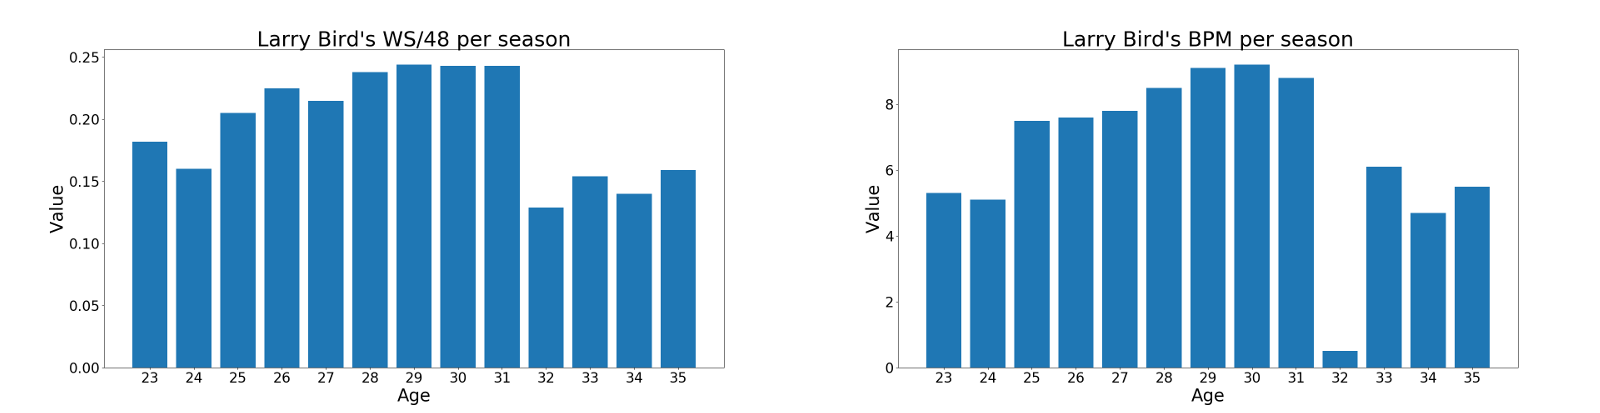
\includegraphics[scale=0.30]{bird.png}
\end{center}
\caption{Bird's WS/48 and BPM per season}
\label{plt:bird}
\end{figure}

\begin{figure}[h!]
\begin{center}
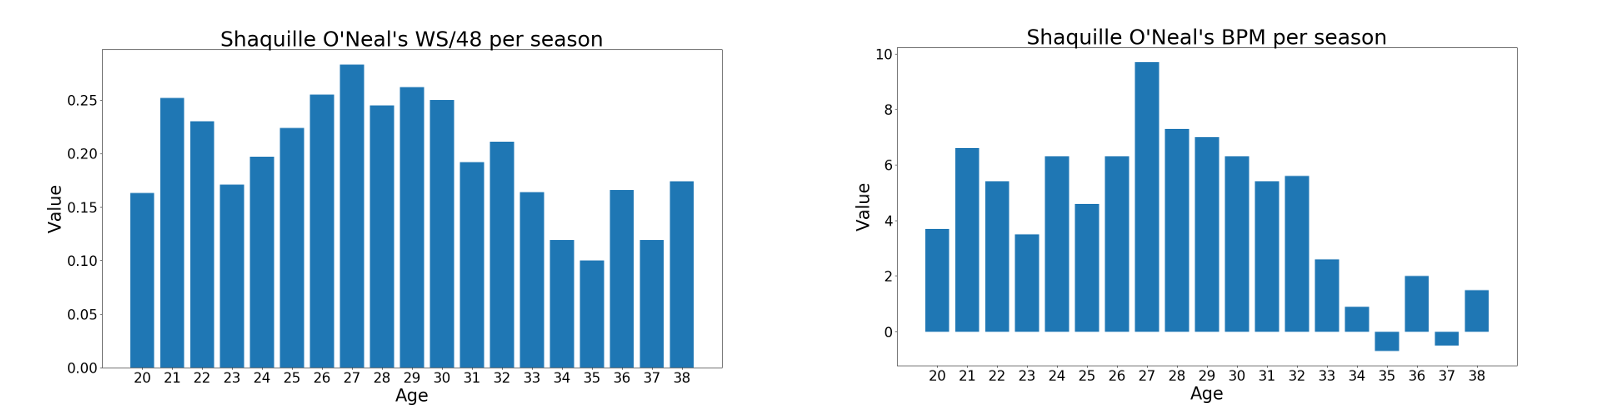
\includegraphics[scale=0.30]{shaq.png} % 2 x 800px and 413px
\end{center}
\caption{Shaq's WS/48 and BPM per season}
\label{plt:shaq}
\end{figure}

\begin{figure}[h!]
\begin{center}
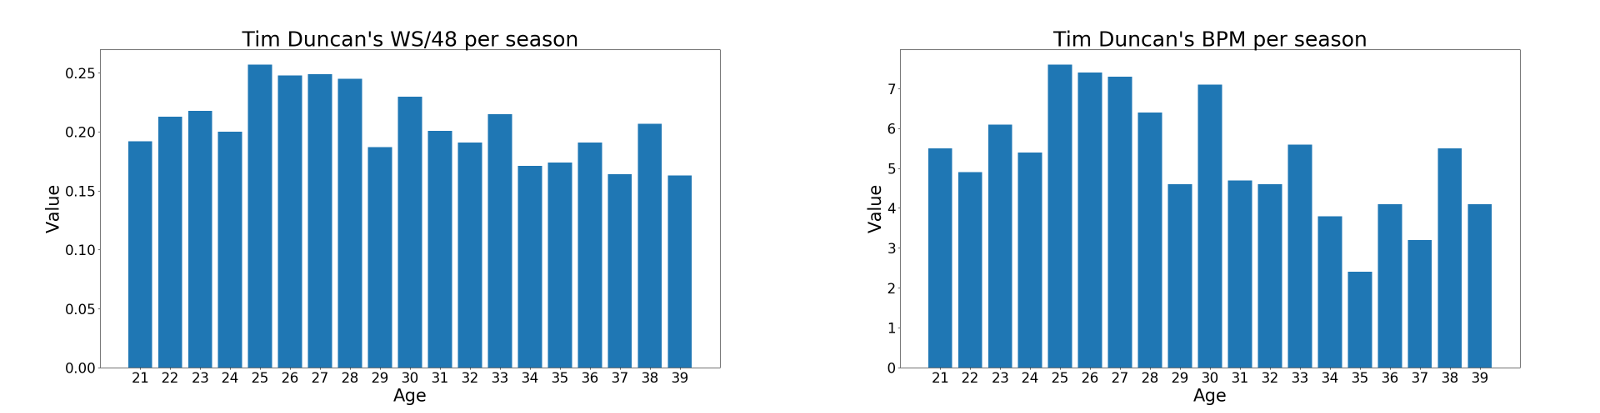
\includegraphics[scale=0.30]{duncan.png}
\end{center}
\caption{Duncan's WS/48 and BPM per season}
\label{plt:duncan}
\end{figure}


In the next step of determining prime of players, I checked at what age do players win awards, such as \textit{Regular season MVP}, \textit{Finals MVP}, \textit{DPOY} and \textit{Sixth man of the year} (\textit{SMOY}). Plots are shown in figure \ref{plt:awards}. Every plot but the plot for Defensive player of the year is somewhat similar. In those plots the number of awards players won while in their late twenties and eary thirties is greater than number of awards in other years. Defensive player of the year award plot is different, where players aged from 23 to 31 won with roughly the same frequency, with an exception of players who were 28 (highest value) and 27 years old when they won. After that, there is a significant drop. These plots are showing us that the best players in the season are usually ones between 26 and 31 years old. But those players are stars and superstars. What about an average player?

\begin{figure}[h!]
\begin{center}
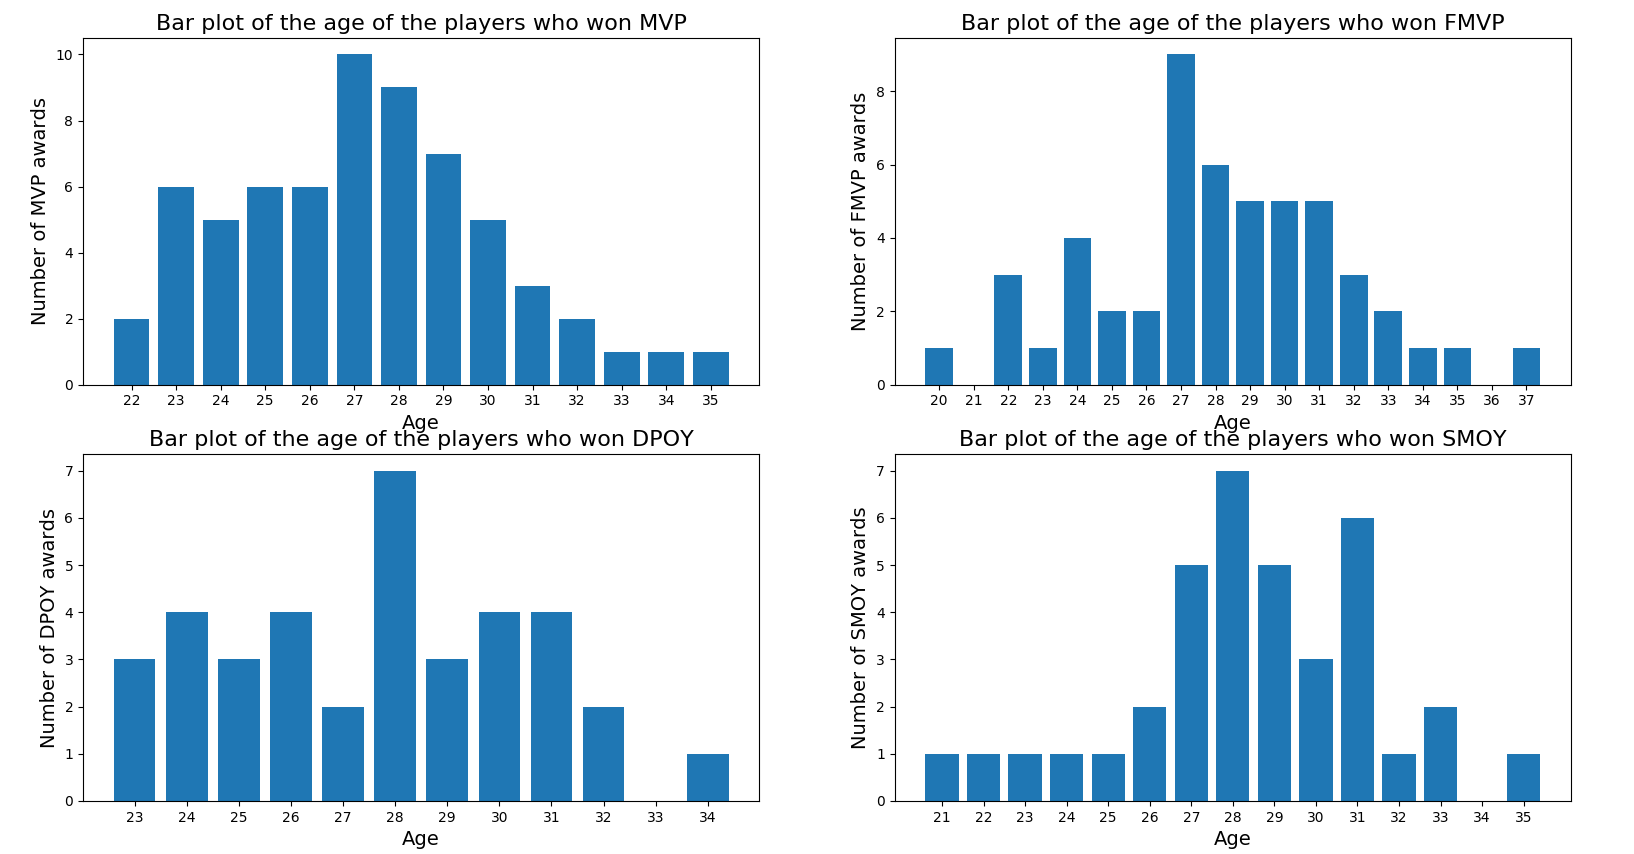
\includegraphics[scale=0.3]{awards_plots.png}
\end{center}
\caption{Age of award winners}
\label{plt:awards}
\end{figure}

After that, I checked age of players who played in the NBA. Results can be seen in figure \ref{plt:age_hist}. Note that there are two histograms. One represents every player who played in the NBA. The other is filtering out every player that has played in less than 35 games and less then 15 minutes per game. Those players are filtered out because I don't consider them regular contributors for the team they are playing for. The reason behind that is that they are probably not skilled enough, and possibly not in their prime, so they might not be important. Also, I just wanted to check on their histogram as well. Data used only takes into account players in the so-called \textit{Three-point era}. which began in 1979/80 season, the first season with 3-point line, and last till this day.

\begin{figure}[h!]
\begin{center}
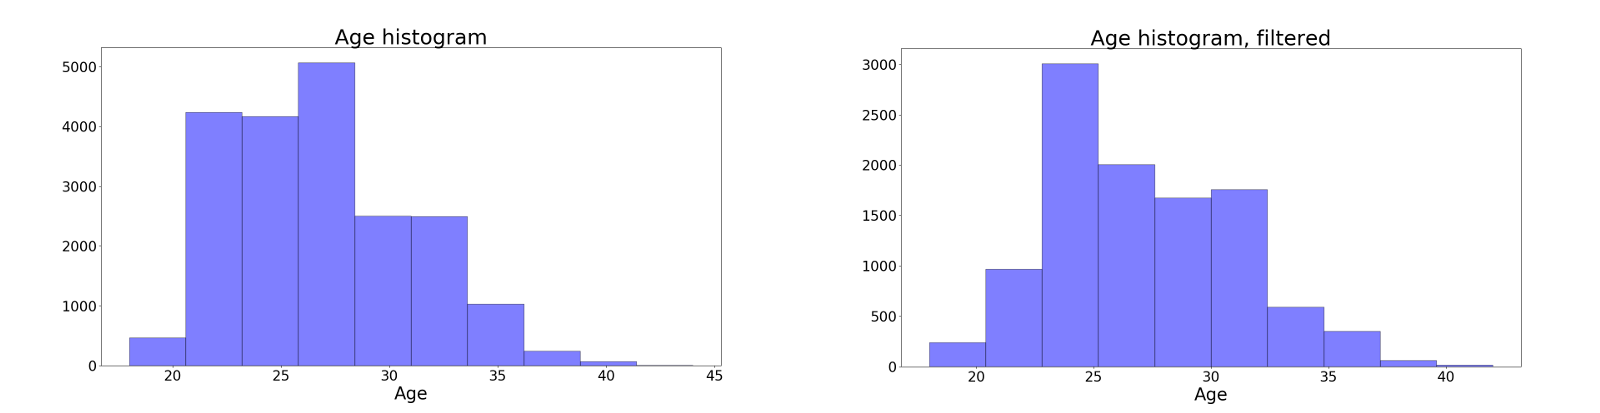
\includegraphics[scale=0.3]{age_histograms.png}
\end{center}
\caption{Age histograms}
\label{plt:age_hist}
\end{figure}


In the left histogram, unfiltered one, most of the players are in between 21 and 28 years old. That makes sense because players are usually drafted when they are younger than 25, and after rookie contracts expire and they are not good enough, they are out of the league. Histogram on the right has way lower number of players youger than around 23 years old. The reason behind that is that rookies aren't usually contributors right away because they need some time to develop.   The difference in number of players that are above 28 years old in unfiltered and filtered data is not that large. That is the case because players obove that age are usually good players, and they might be good because they are in their prime. That trend continues on both histograms until the significant drop somewhere after players reach 32 or 33. That might happen because they are simply not serviceable anymore, and because of that cannot find teams to sign with. 
To conclude this paragraph, number of players is rising ar first, until the age of 28 (or 25 for filtered players). After that, there are two significant drops.

Now, I can try to estimate prime of an average player with statistics. First, I checked traditional stats. Bar plots for four stats are shown, PTS, FG, FGA and FT. Simply, it is expected from a player in his prime to shoot and score more than in his non-prime seasons. Note that values represented on a y-axis are averages per season, not per game! In figure \ref{plt:totals_age} every player from the three-point era is taken into account while players represented in the figure \ref{plt:totals_age_filtered} are the ones I consider contributors (minutes per game $>$ 15 and games played $>$ 35).

\begin{figure}[h!]
\begin{center}
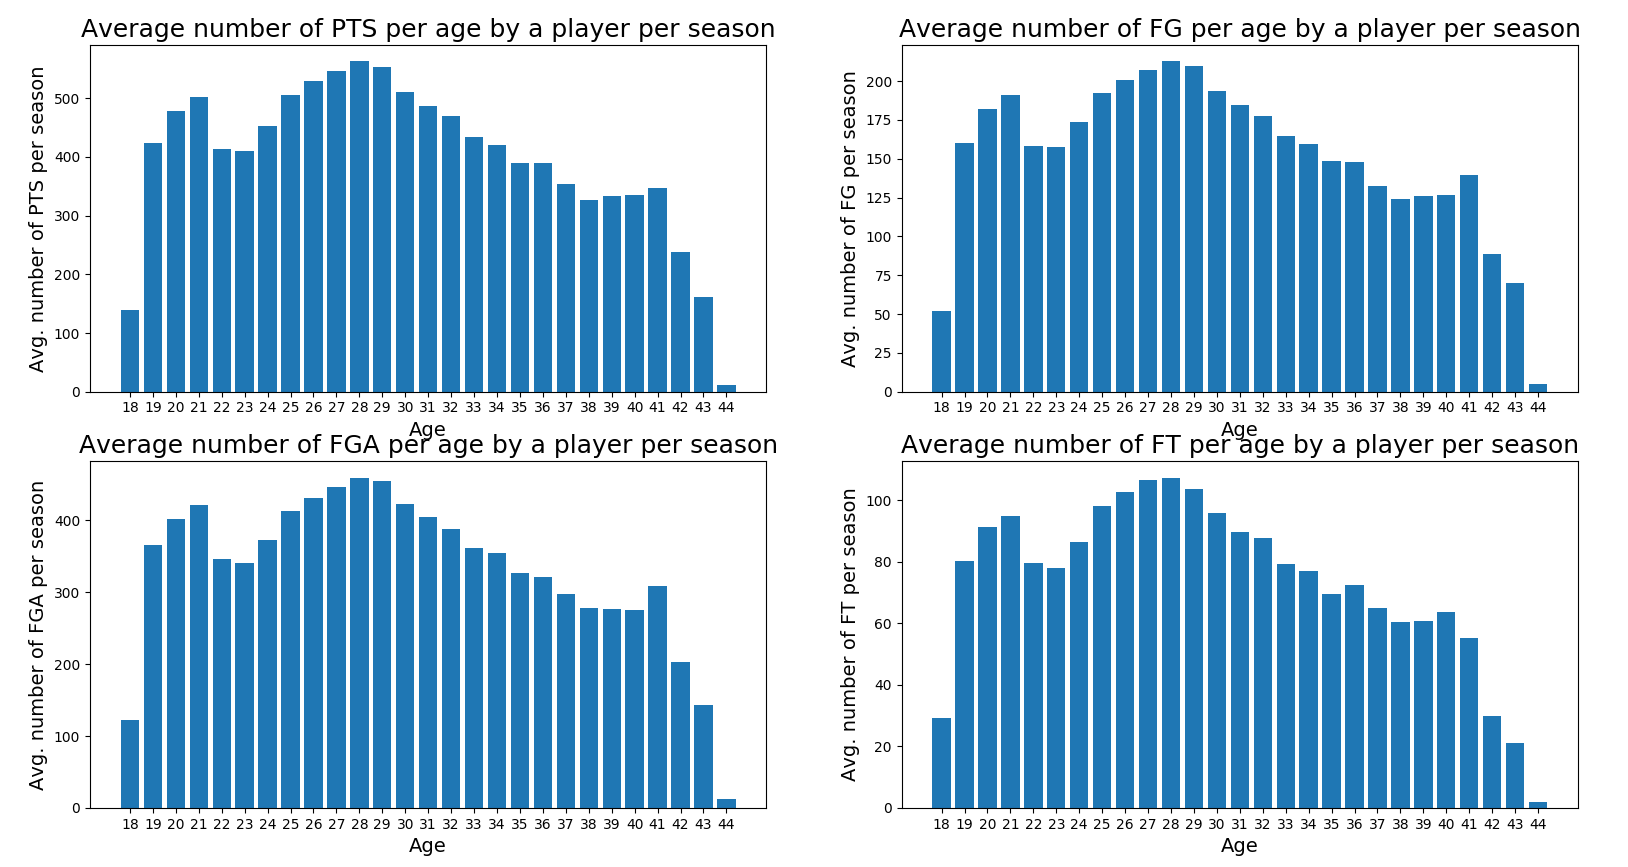
\includegraphics[scale=0.3]{traditional_stats_per_age.png}
\end{center}
\caption{Season totals averages per age unfiltered}
\label{plt:totals_age}
\end{figure}

\begin{figure}[h!]
\begin{center}
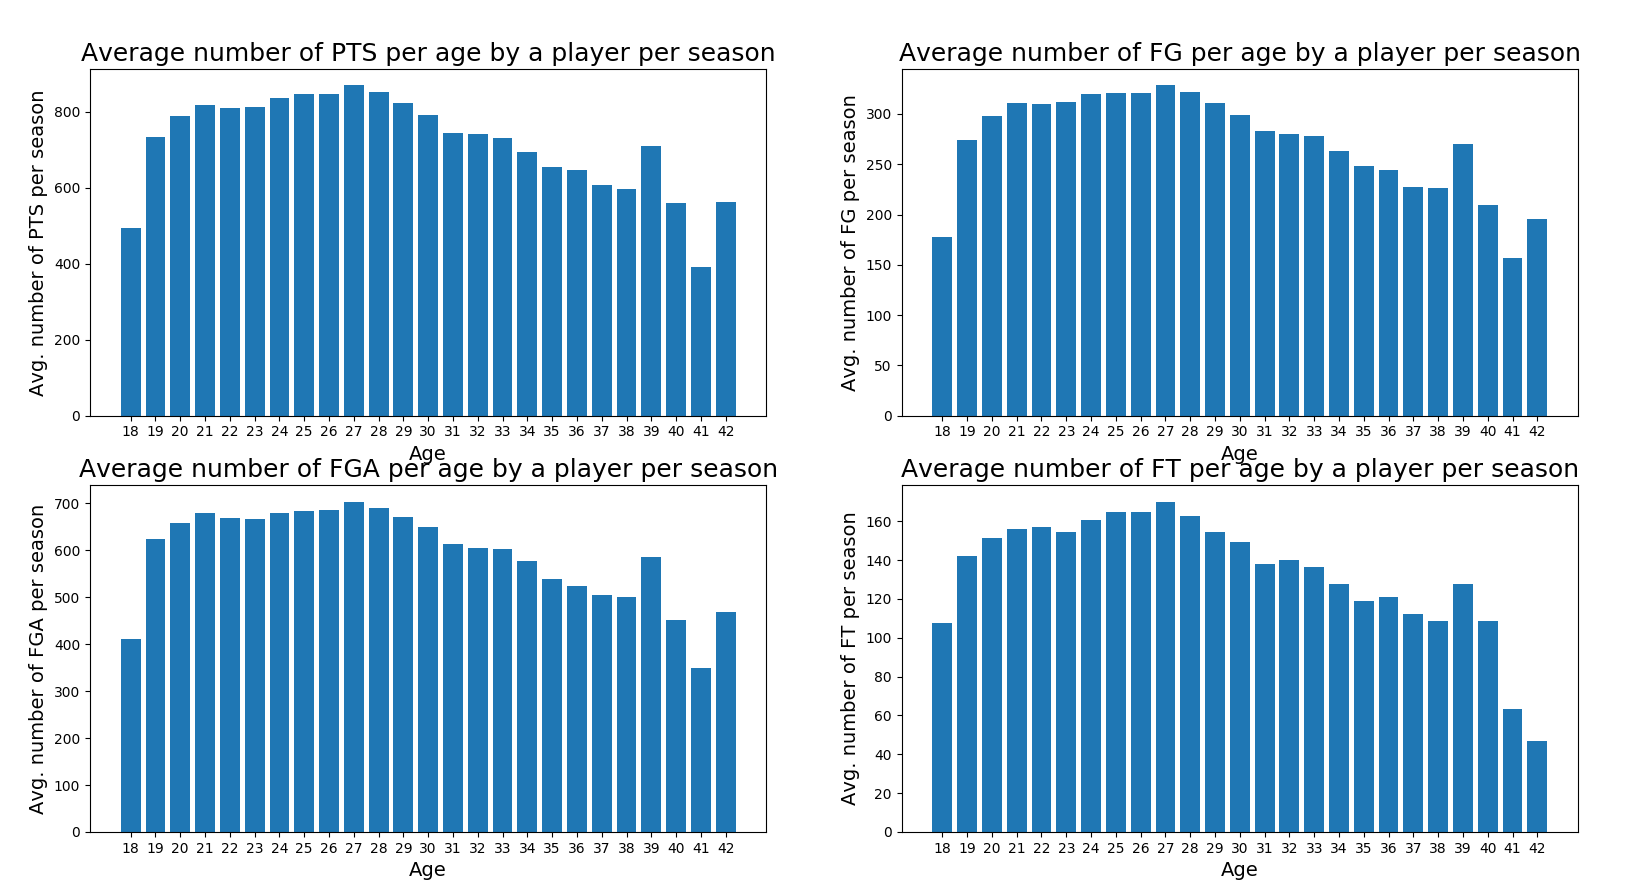
\includegraphics[scale=0.3]{traditional_stats_per_age_filtered.png}
\end{center}
\caption{Season totals averages per age filtered}
\label{plt:totals_age_filtered}
\end{figure}

Both figures are somewhat similar. Values for players age from 26 to 30 or maybe 31 are higher than for any other age, with a significant drop after that. Both figures show peaks at a similar age, 28 for unfiltered data and 27 for filtered. So it's good thing to consider that prime of an average player is acually in late twenties/early thrties. The main difference can be seen in values for players that are younger than 25. Unfiltered data has easily noticable difference between values for players 21 and players 22 years old. Reason behind that is probably draft. Promising players are drafted earlier, often before they are 20, while a lot of players with lower upside decide to devlop in college and try to enter the league later. Those players are the reason why the values are lower for certain age. From plots with filtered data we can observe that those players are not contributing right away, so lower values are, while still there, not so emphasized.

Advanced stats are better than traditional and hold more information about how good a certain player is. So, I did similar thing as in the paragraphs before, but now with the advanced stats. Stats chosen are PER, WS, BPM and VORP. Bar plots for unfiltered players are shown in figure \ref{plt:advanced_age}, while bar plots after filtering are in figure \ref{plt:advanced_age_filtered}.


\begin{figure}[h!]
\begin{center}
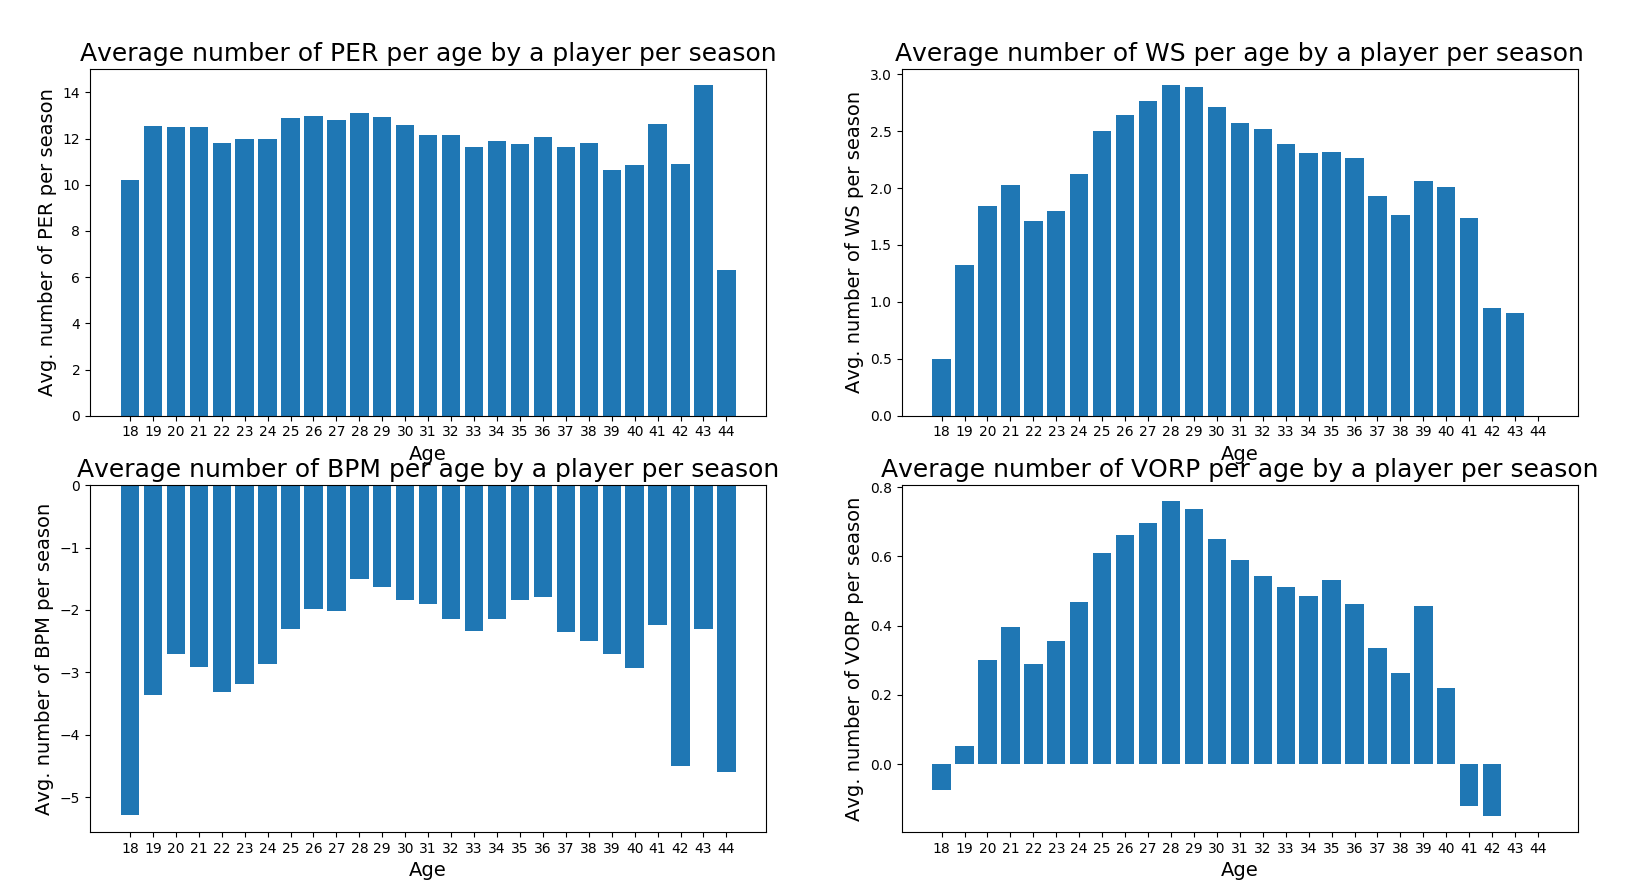
\includegraphics[scale=0.3]{advanced_stats_per_age.png}
\end{center}
\caption{Advanced stats averages per age unfiltered}
\label{plt:advanced_age}
\end{figure}

\begin{figure}[h!]
\begin{center}
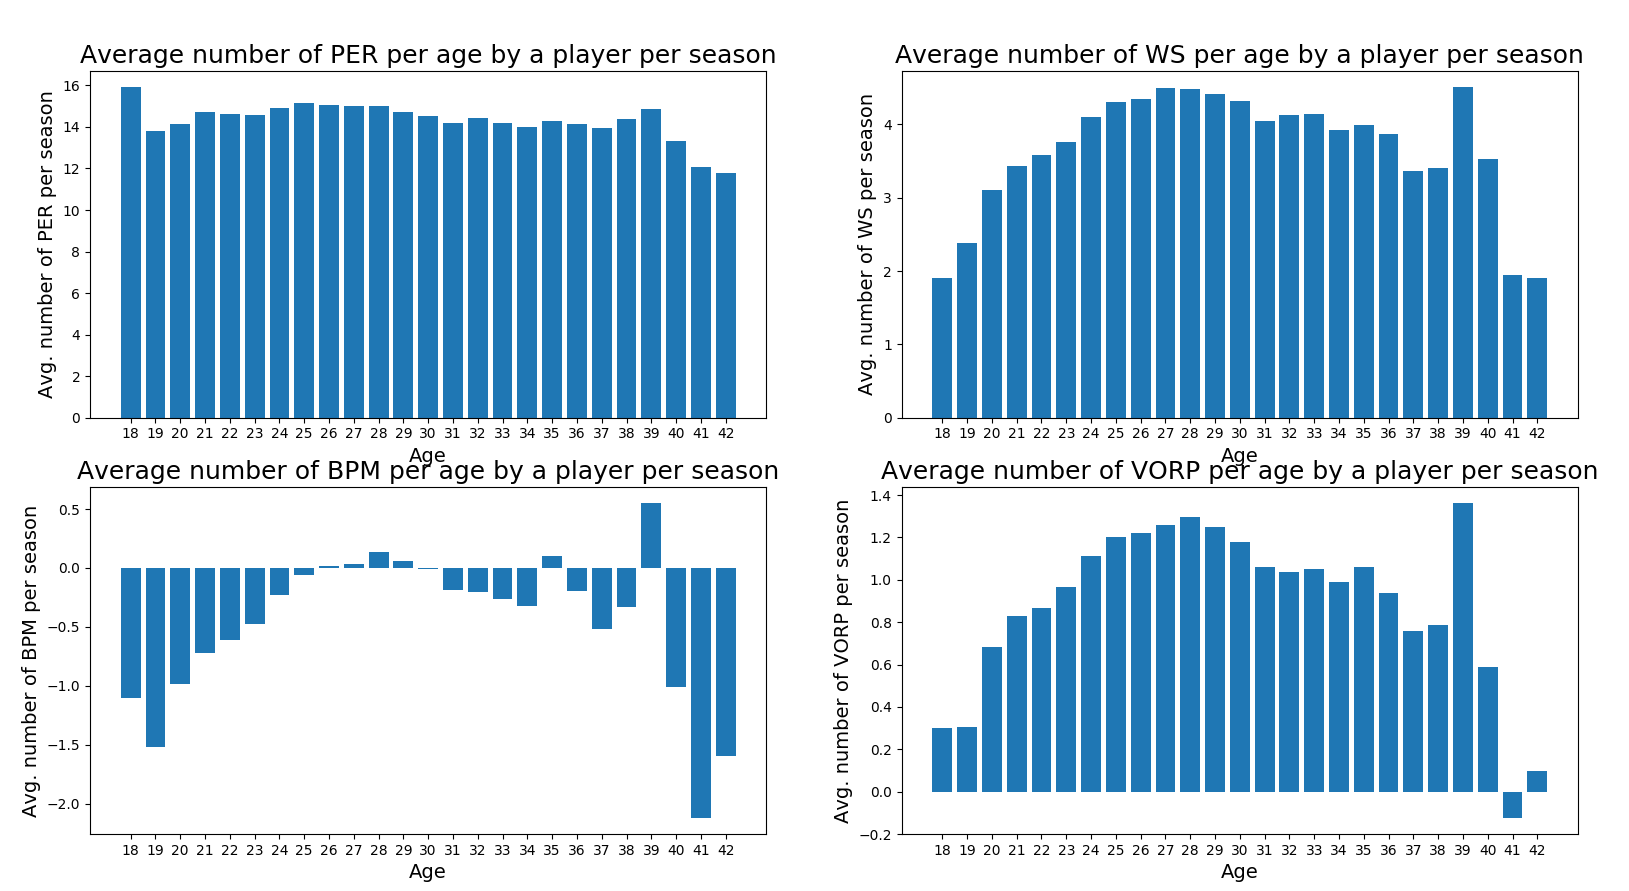
\includegraphics[scale=0.3]{advanced_stats_per_age_filtered.png}
\end{center}
\caption{Advanced stats averages per age filtered}
\label{plt:advanced_age_filtered}
\end{figure}

These plots are way more interesting. First, PER bar plot, for both fitered and unfiltered data, is somewhat similar to the ones with traditional stats, with the same results. Plots for WS and VORP are \textbf{normal distribution-like}, with spike from 26 to 31 in y-axis values and lower values from the sides. That radius with higher values contains prime years af an average player. Plot for BPM is, interestinglly, negative for unfiltered data, and with some possitive values for filtered data. Highest values for BPM are from players from 25 to 36 years old. Some of the plots that are showing advanced data have high value for players 39 years old, wich is interesting. Those players were usually very good in their prime, and because of that they were usually good when they were older, just not that good anymore, and in usually lower minutes per game. Also, not many players play by that age, so the average might be high because there is a small number of players, none of which are bad.

Taking all mentioned things into a consideration, age when players are usually winning awards and age when the players are statistically better than in any other age, conclusion is that an average player enters into prime at around his \textbf{25th} year, and exits when he is around \textbf{31}, with kinda significant drop after that. Peak season happens when player is from \textbf{27 to 29} years of age, somewhere in the middle of their prime.

\section{Nikola Joki\' c analysis}
\label{jokic}

Nikola Jokić was drafted by the Denver Nuggets as a 41st overall pick in the 2014 NBA draft. One year later, he signed with the team, and soon became the starting center, and the team's best player. Let's see some of his stats per season through his career. Traditional stats are shown in the figure \ref{plt:trad_jokic} while advanced stats are shown in figure \ref{plt:adv_jokic}.

\begin{figure}[h!]
\begin{center}
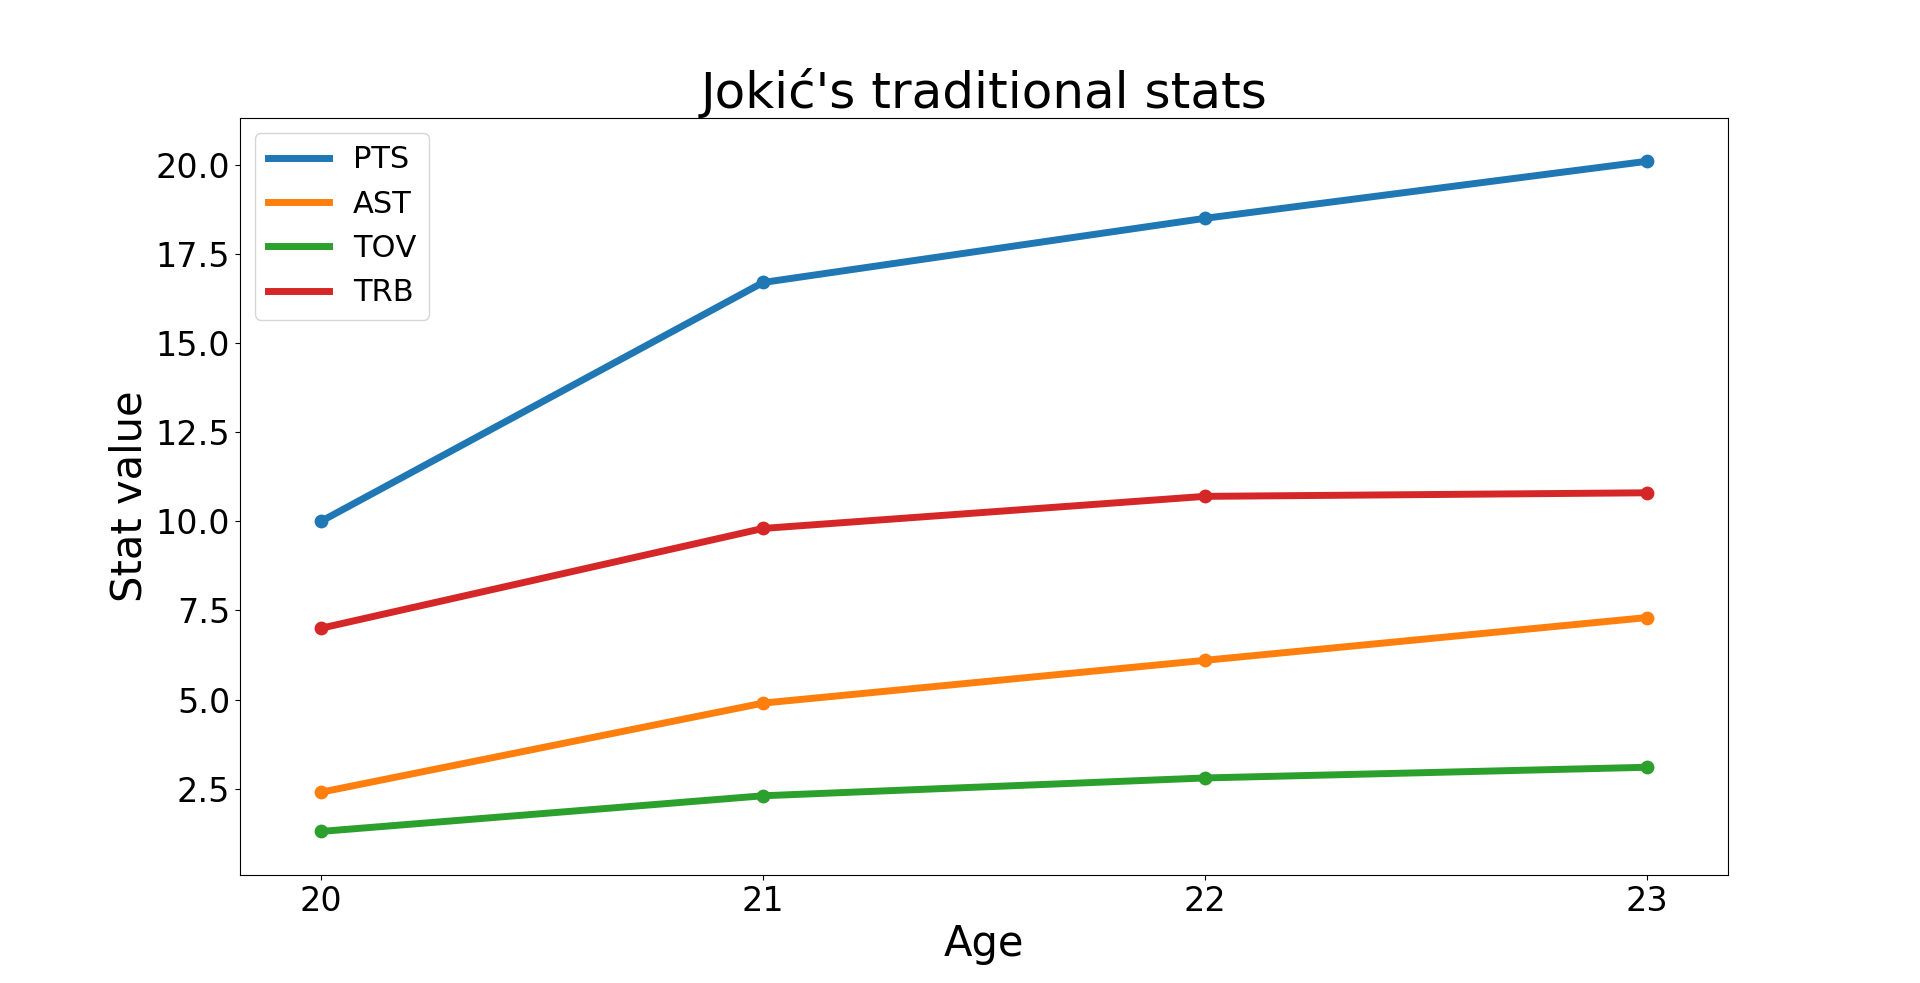
\includegraphics[scale=0.25]{jokic_plot_traditional.png}
\end{center}
\caption{Traditional stats by Joki\' c per season}
\label{plt:trad_jokic}
\end{figure}

\begin{figure}[h!]
\begin{center}
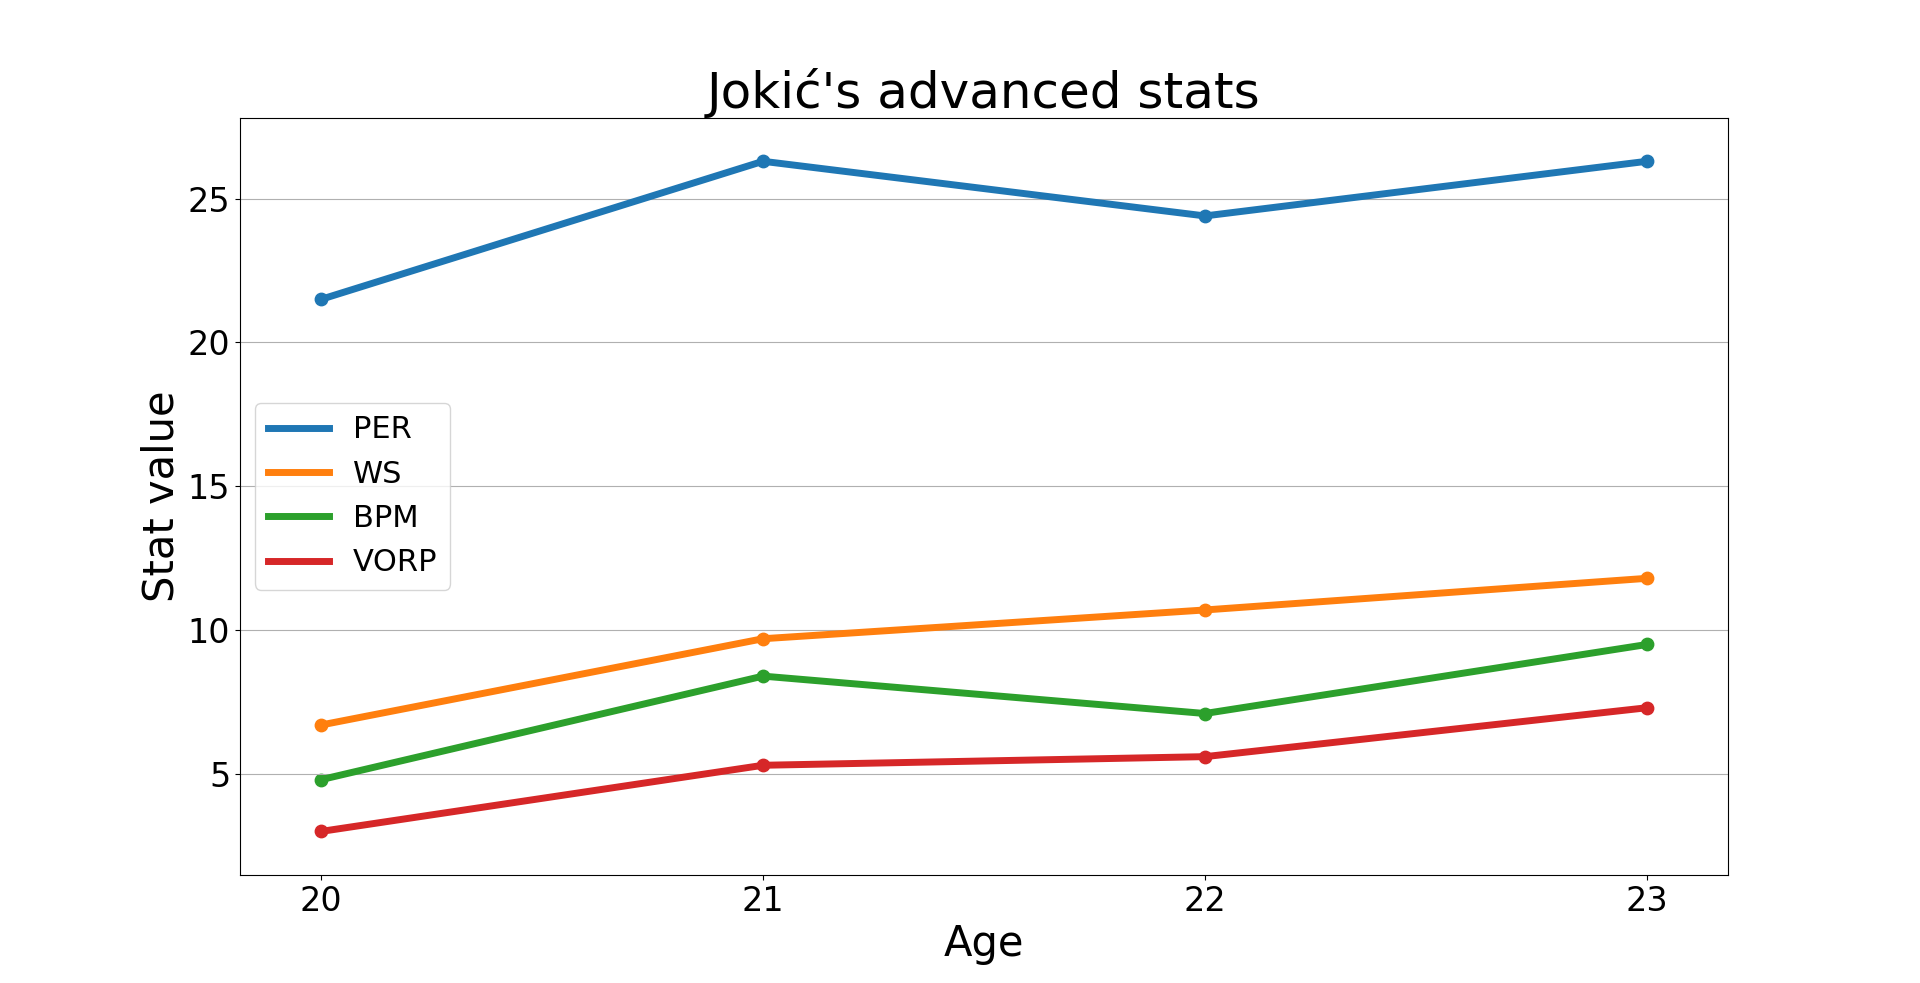
\includegraphics[scale=0.25]{jokic_plot_advanced.png}
\end{center}
\caption{Advanced stats by Joki\' c per season}
\label{plt:adv_jokic}
\end{figure}

As we can see, the stats are getting better as he age, and are very good in his forth season (2018-19) where he earned spot on the \textbf{1st All-NBA} team and the \textbf{All-star} selection.

\subsection{Did he deserve 1st team All-NBA in the 18-19 season?}
\label{subsec:jokic_all_nba}

Let's start this subsecion with a note that All-NBA teams are \textit{selected by voters}, and \textbf{not} purely by stats. That means that the players who are statistically very good might not get All-NBA team selection, if, for example, a team they play for isn't successful, although that's unlikely. Also, player doesn't have to be one of the five best players in the league to end up on the 1st All-NBA team, he just have to be the best, according to a voter, at his position. The All-NBA team consists of two guards, two wings and one center. In the 2018-19 season, Nikola Joki\' c was on the 1st All-NBA team. Did he \textit{statistically} deserve it?

Joki\' c is a \textit{center}, and there is only one center on the 1st All-NBA team, so I just have to compare his stats with the stats of the other centers. In the 2018-19 season, Joki\' c played in 80 games, averaging 31.3 MPG, 20.1 PPG, 10.8 RPG and 7.3 APG on 0.51 FG\%, 0.31 3P\%, 0.82 FT\% shooting splits. Here is how it compared to other \textbf{centers} in the same season. Plot chosen to represent this data is Box plot \cite{boxplots}, because we want to see whether Joki\' is, and how much, better than other centers.


\begin{figure}[h!]
\begin{center}
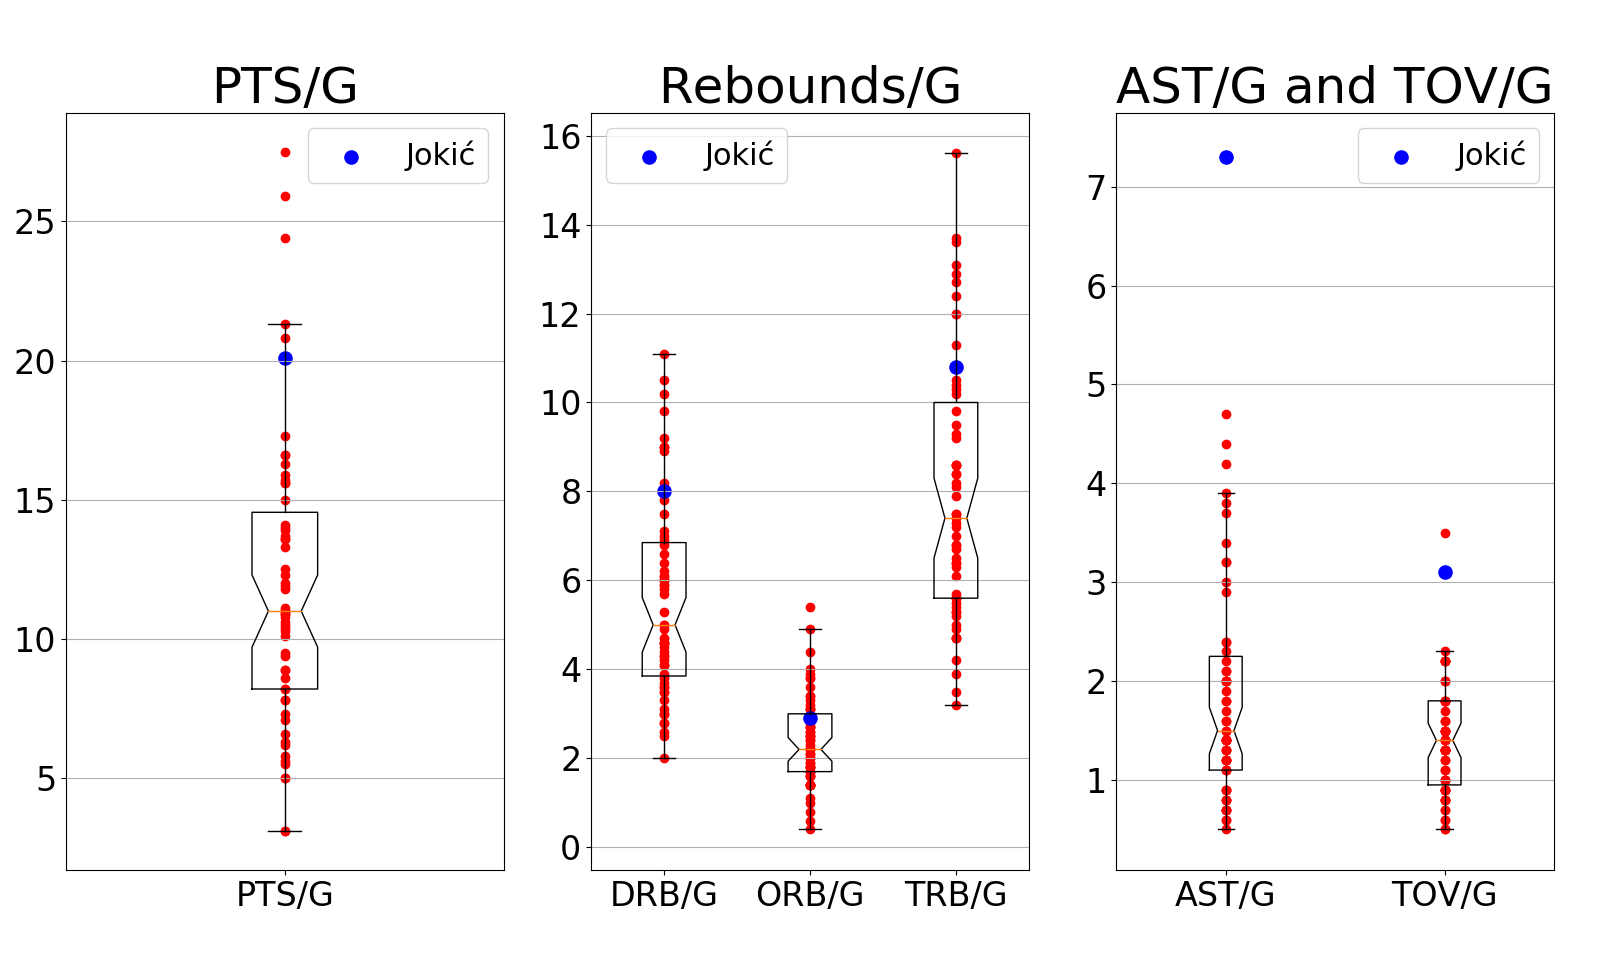
\includegraphics[scale=0.30]{centers_traditional.png}
\end{center}
\caption{Box plots of the traditional stats by centers in 2018-19 season}
\label{plt:centers_trad}
\end{figure}

These stats are showing that Joki\' c really was one of the best centers in the league. Although not the best scorer or rebounder (but still very good), he had by far the most assists, almost three more than the second placed Marc Gasol, which is probably the reason why he had the 2nd most turnovers. As we have seen, traditional stats are almost always inferior to advanced when evaluating how good a certain player is. That is why the next step is to check out Joki\' c's, (figures \ref{plt:centers_adv} and \ref{plt:centers_bpm}) and compare it with others.

\begin{figure}[h!]
\begin{center}
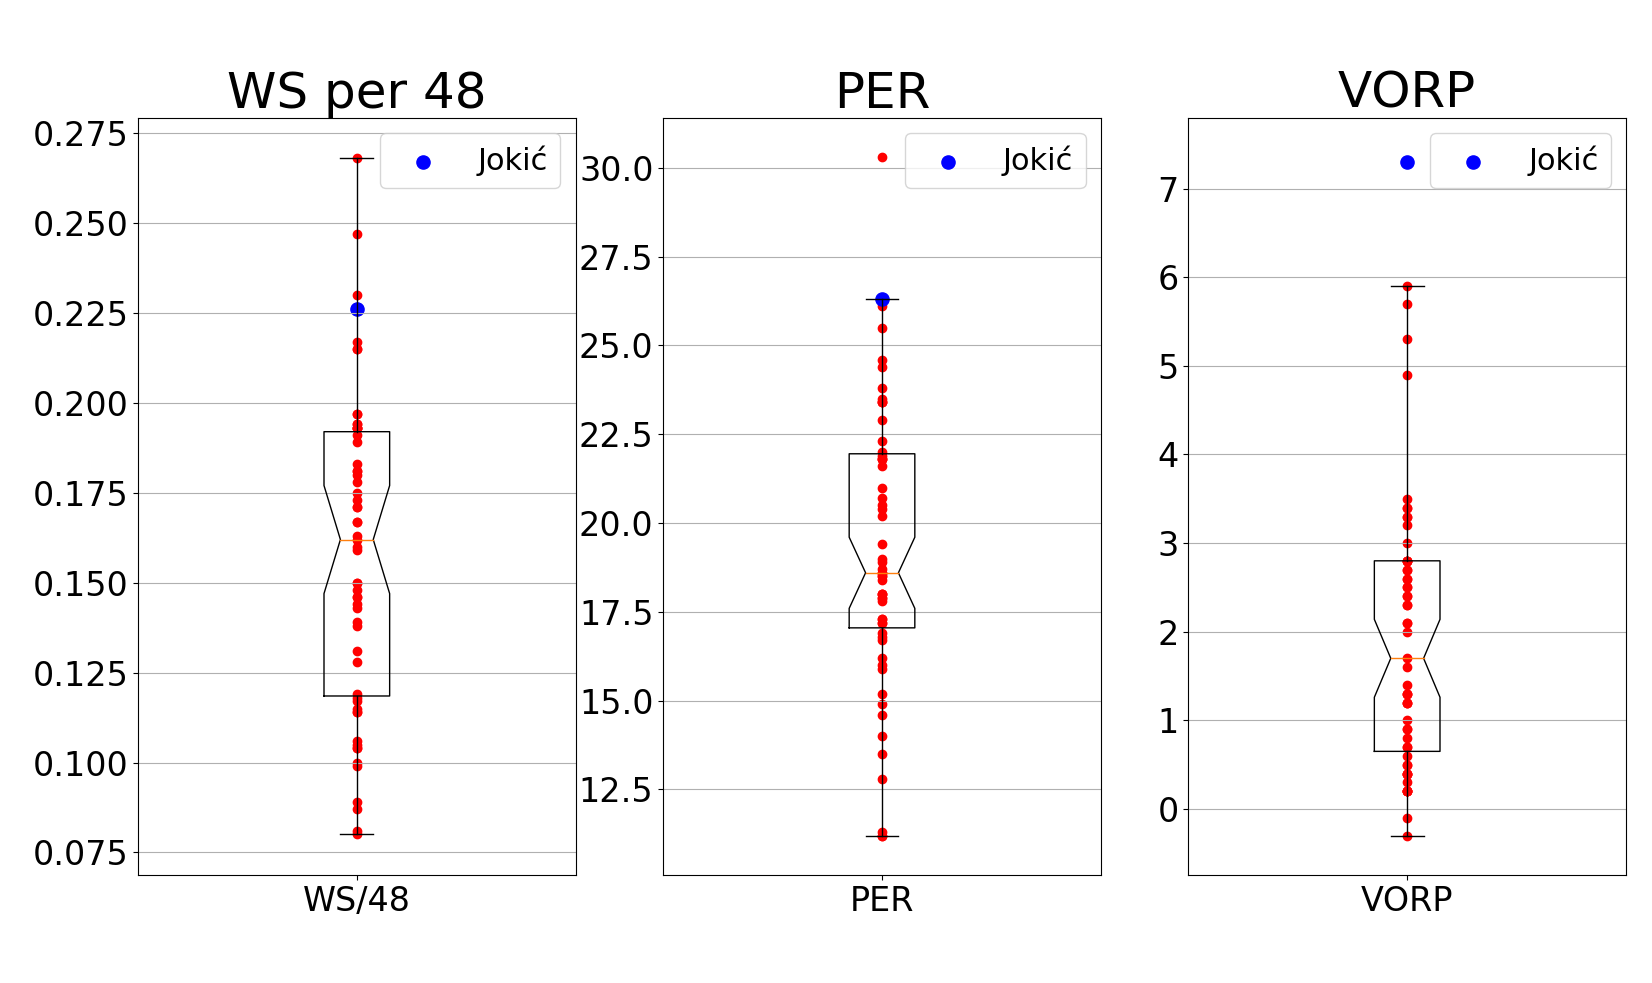
\includegraphics[scale=0.30]{centers_advanced.png}
\end{center}
\caption{Box plots of the advanced stats by centers in 2018-19 season}
\label{plt:centers_adv}
\end{figure}

\begin{figure}[h!]
\begin{center}
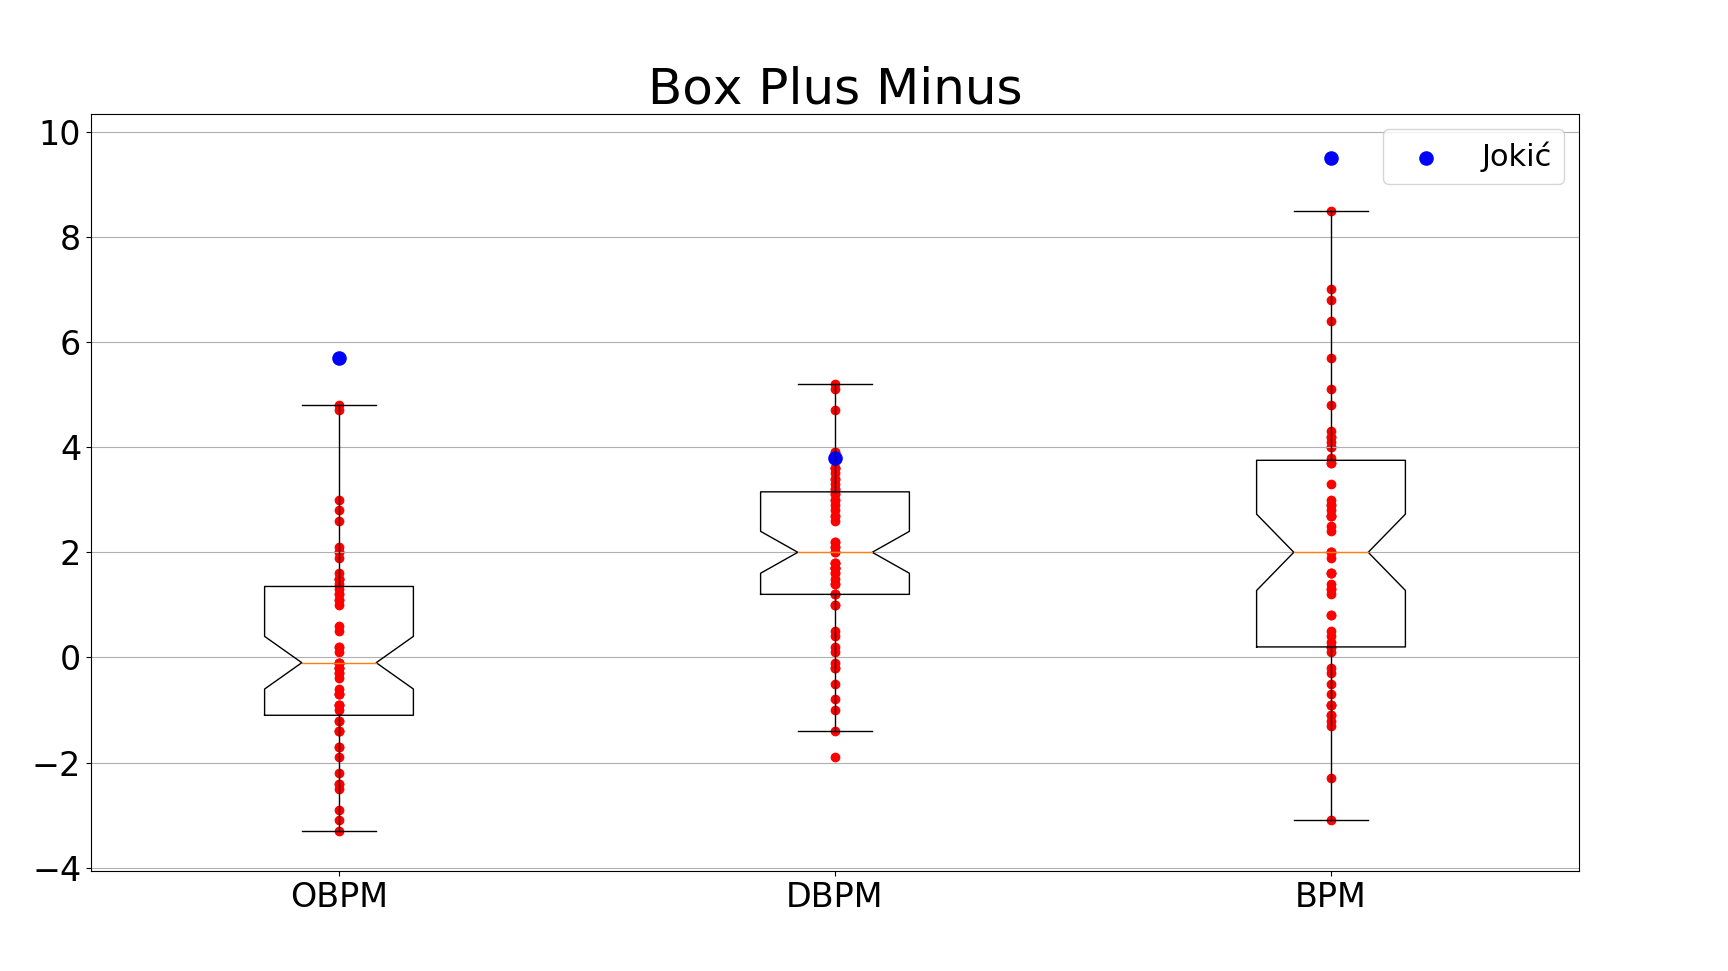
\includegraphics[scale=0.30]{centers_bpm.png}
\end{center}
\caption{Box plots of the Box Plus Minus stats by centers in 2018-19 season}
\label{plt:centers_bpm}
\end{figure}

Among centers, he was ranked high on WS/48 (4th), PER (2nd) and DBPM (5th) and is \textbf{first} in VORP (3rd in the league), OBPM (7th in the league) and BPM (3rd in the league). He dominated advanced statistics, not only when compared to the other players at his position, but also when compared to the best players in the NBA in that season. From this, it is not hard to determine that Nikola Joki\' c statstically deserved to be on the All-NBA 1st team! Of course, that does not mean that other centers weren't, but it means that voters had good reasoning behind their decision. The thing that certainly helped was that Denver Nuggets, led by him as the best player, were 2nd seeded team in the Western conference.

\subsection{Passing}
\label{subsec:jokic_passing}

The thing Joki\' c is most known for is definitely his passing ability, the thing the average center isn't. In this subsection I will take a look at his passing statistics, and compare it to other players (not just centers) from the NBA history. But first, let's see how his passing compares to the other centers. As we have seen in the previous subsection, his AST/G number (7.3) was by far the best in the league at his position. How many centers in the history averaged something similar? Table \ref{tab:centers_ast_g} contains every season where a center averaged more than  six AST per game. 

\begin{table}[h!]
\begin{center}
\begin{tabular}{|c|c|c|c|c|} \hline
\textbf{Player} & \textbf{Age} & \textbf{Season} & \textbf{Minutes per game} & \textbf{Assists per game} \\ \hline
Wilt Chamberlain & 31 & 1967-68 & 46.8 & 8.6 \\ \hline
Wilt Chamberlain & 30 & 1866-67 & 45.5 & 7.8\\ \hline
Nikola Jokić & 23 & 2018-19 & 31.3 & 7.3 \\ \hline
Nikola Jokić & 22 & 2017-18 & 32.6 & 6.1 \\ \hline
\end{tabular}
\caption{Centers with more than six assists per game in a season}
\label{tab:centers_ast_g}
\end{center}
\end{table}

Yes, only two centers in the \textbf{history} of the NBA menaged to average more than six assists per game in a season. Number of seasons with decreased AST/G in a season by a center, \textbf{five}, is 21, by only 13 players. Wilt Chamberlain appears on this expanded list four times, ranked 1st, 2nd, 15th, 20th, while number of Nikola Joki\' c such seasons remains the same, two, with 3nd and 4th spots. Note that Joki\' c's third highest AST/G is 4.9, so he misses new list by a tiny margin.

The best way to compare players would be per possession stats, but those stats were measured from 1973-74 season, some seasons after Wilt set his personal record in AST/G. Instead of that we can only compare per minute production (table \ref{tab:jokic_wilt_per_36}). In this category, Joki\' c is better than Chamberlain, with the significant difference. Note that there are 5 centers (9 seasons in total), that played more than 15 MPG and 35 G in a season and menaged to average more than six AST per 36, with Joki\' c being the first on that list, and only one with more than seven AST per 36. He is also 4th and 7th, while Chamberlain takes 5th and 8th spots.

\begin{table}[h!]
\begin{center}
\begin{tabular}{|c|c|c|c|c|} \hline
\textbf{Player} & \textbf{Age} & \textbf{Season} & \textbf{Minutes per game} & \textbf{Assists per 36} \\ \hline
Nikola Jokić & 23 & 2018-19 & 31.3 & 8.3 \\ \hline
Nikola Jokić & 22 & 2017-18 & 32.6 & 6.7 \\ \hline
Wilt Chamberlain & 31 & 1967-68 & 46.8 & 6.6 \\ \hline
Wilt Chamberlain & 30 & 1866-67 & 45.5 & 6.2 \\ \hline
\end{tabular}
\caption{Joki\' c's and Chamberlain's AST per 36 minutes}
\label{tab:jokic_wilt_per_36}
\end{center}
\end{table} 

Not only Joki\' c has hight AST per 36 minutes number, he is also at the top for AST per 100 possessions stat. In fact, out of top five AST per 100 seasons by a center (table \ref{tab:centers_ast_per100_top5}), Joki\' c has three! He is ranked 1st, 3rd and 5th. He is also the only center with more than 10 AST per 100, with 11.4, a significant diference to a second-placed Vlade Divac. Note that Joki\' c's rookie season, although not elite, still cracks top 100, at 90th spot.

\begin{table}[h!]
\begin{center}
\begin{tabular}{|c|c|c|c|c|} \hline
\textbf{Player} & \textbf{Age} & \textbf{Season} & \textbf{Assists per 100} \\ \hline
Nikola Jokić & 23 & 2018-19 & 11.4 \\ \hline
Vlade Divac & 35 & 2003-04 & 9.6 \\ \hline
Nikola Jokić & 22 & 2017-18 & 9.3 \\ \hline
Sam Lacey & 31 & 1979-80 & 8.9 \\ \hline
Nikola Jokić & 21 & 2016-17 & 8.6 \\ \hline
\end{tabular}
\caption{Best 5 of AST per 100 possessions by a center}
\label{tab:centers_ast_per100_top5}
\end{center}
\end{table}

High number of assists migh not mean much, if a player turnovers the ball often. When compared to the other centers in TOV per 100 possessions, Joki\' c worst season (2018-19), at 4.9 TOV per 100, is ranked 59th, and it is his only season in the worst 100. This proves that Joki\' c might be \textbf{the best passing big man ever}. But what about other possitions?

First, I compared his stats from 2018-19 to the ones of the other players from the same season. Result can be seen in figure \ref{plt:ast_tov_g}. Bottom right corner is good, top left corner is bad. Not only he is among the best passers in the league, but he is mostly surrounded by point-guards.

\begin{figure}[h!]
\begin{center}
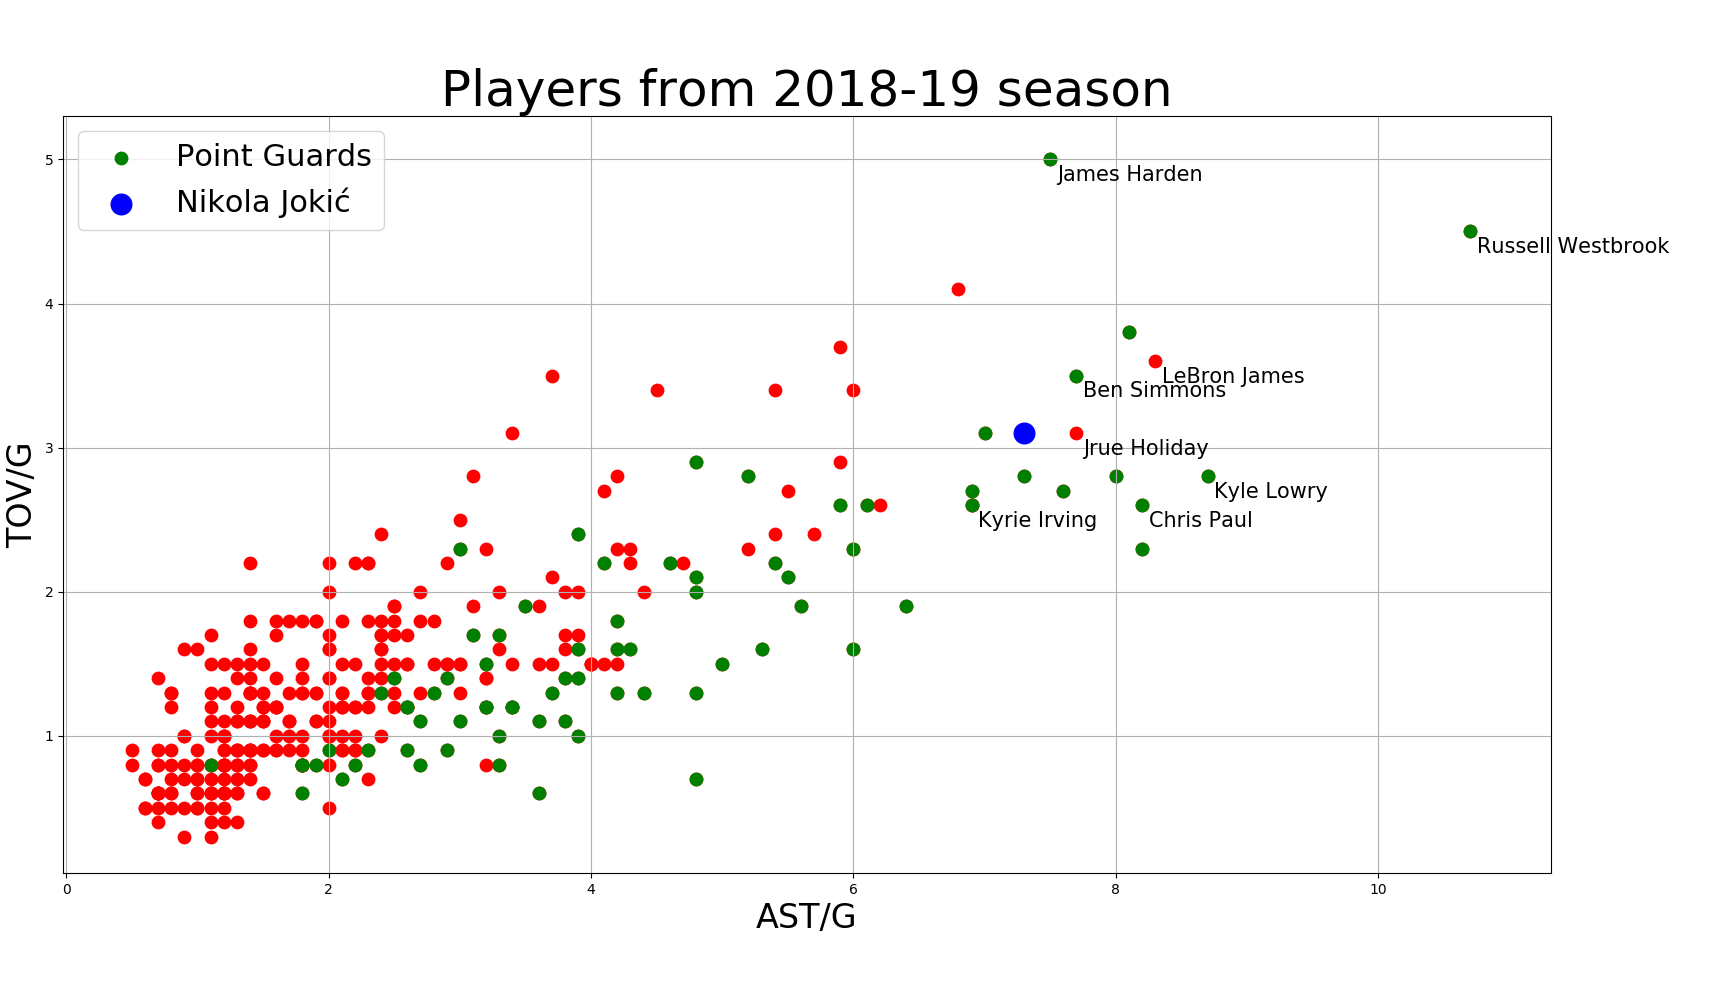
\includegraphics[scale=0.30]{ast_tov_g_2019.png}
\end{center}
\caption{AST/G to TOV/G for players from 2018-19 season (min 15 MP/G and 35 G)}
\label{plt:ast_tov_g}
\end{figure}

The figure \ref{plt:ast_tov_pct} is showing similar results, just this time, instead of AST and TOV per game, AST\% and TOV\% are used. Joki\' c had really good passing season, not just for a center, but overall!

\begin{figure}[h!]
\begin{center}
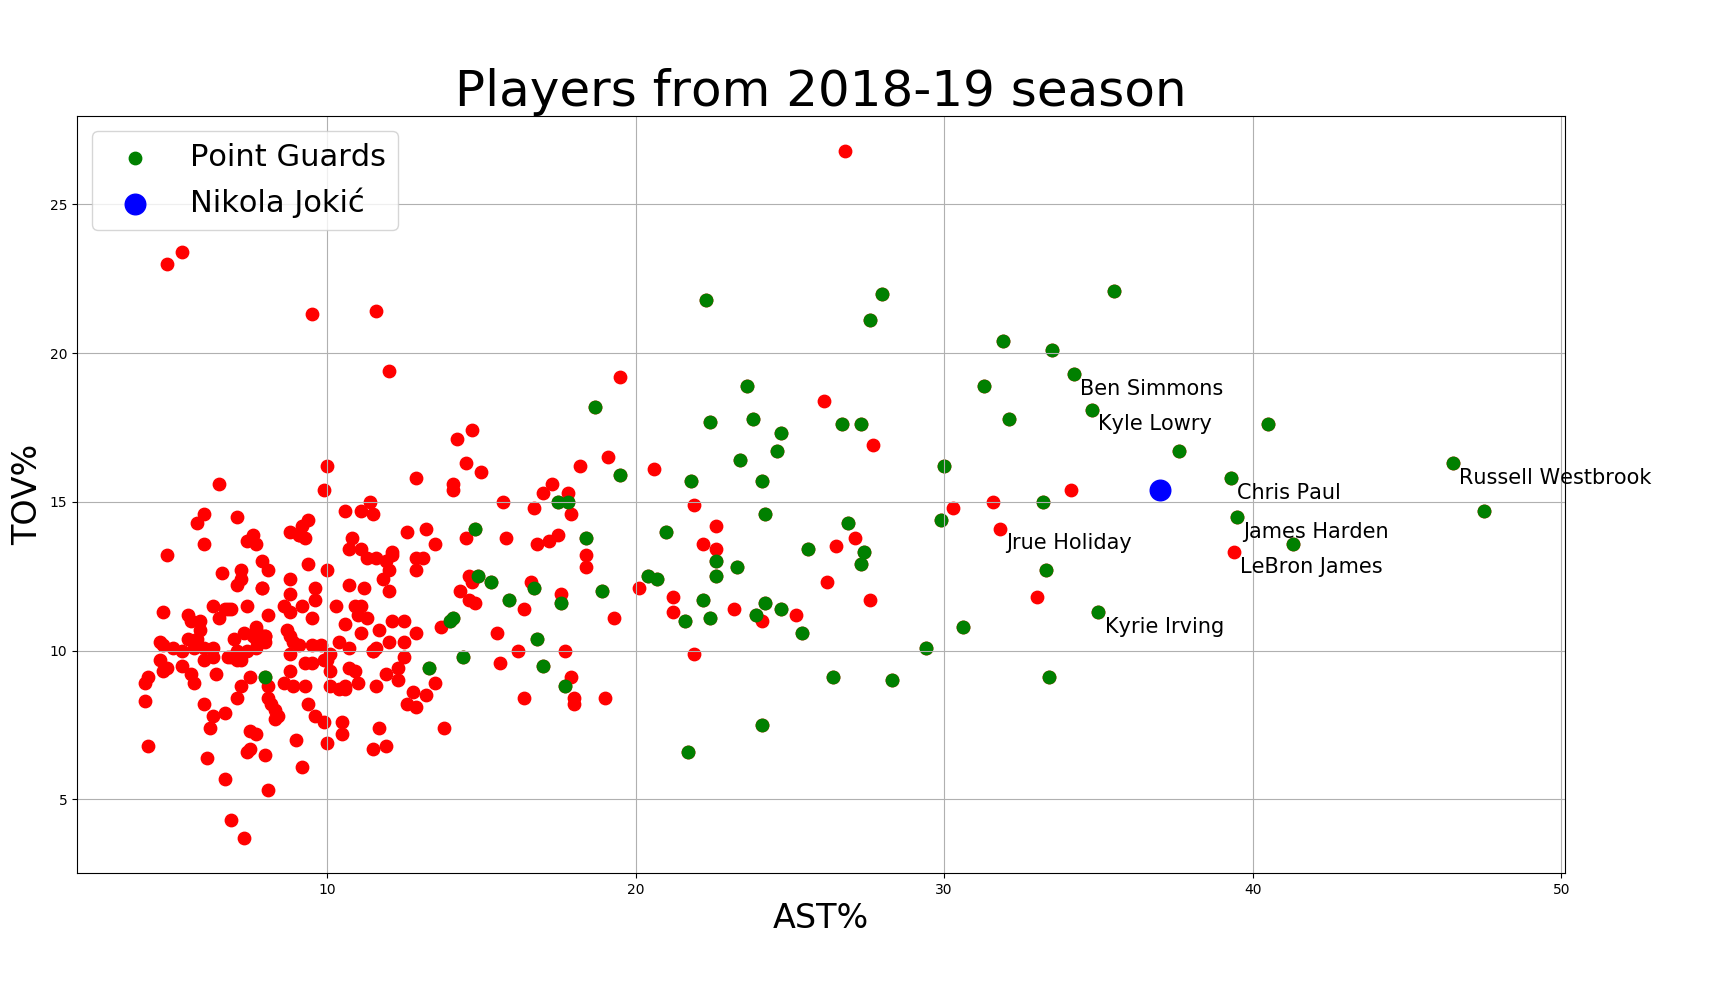
\includegraphics[scale=0.30]{ast_tov_pct_2019.png}
\end{center}
\caption{AST\% to TOV\% for players from 2018-19 season (min 15 MP/G and 35 G)}
\label{plt:ast_tov_pct}
\end{figure}

But what about NBA history? Let's take his best passing season and see how good it was compared to the every player from the 3-point era (figure \ref{plt:ast_tov_g_3p}). This is just the proof that his passing numbers are not center-like. His surroundings are made of non-centers exclusively. Plot is constructed in a way that it is good to be down and right, and bad to be up and left. Joki\' c is somewhere in the middle. That means that his numbers are not elite, but still solid.

\begin{figure}[h!]
\begin{center}
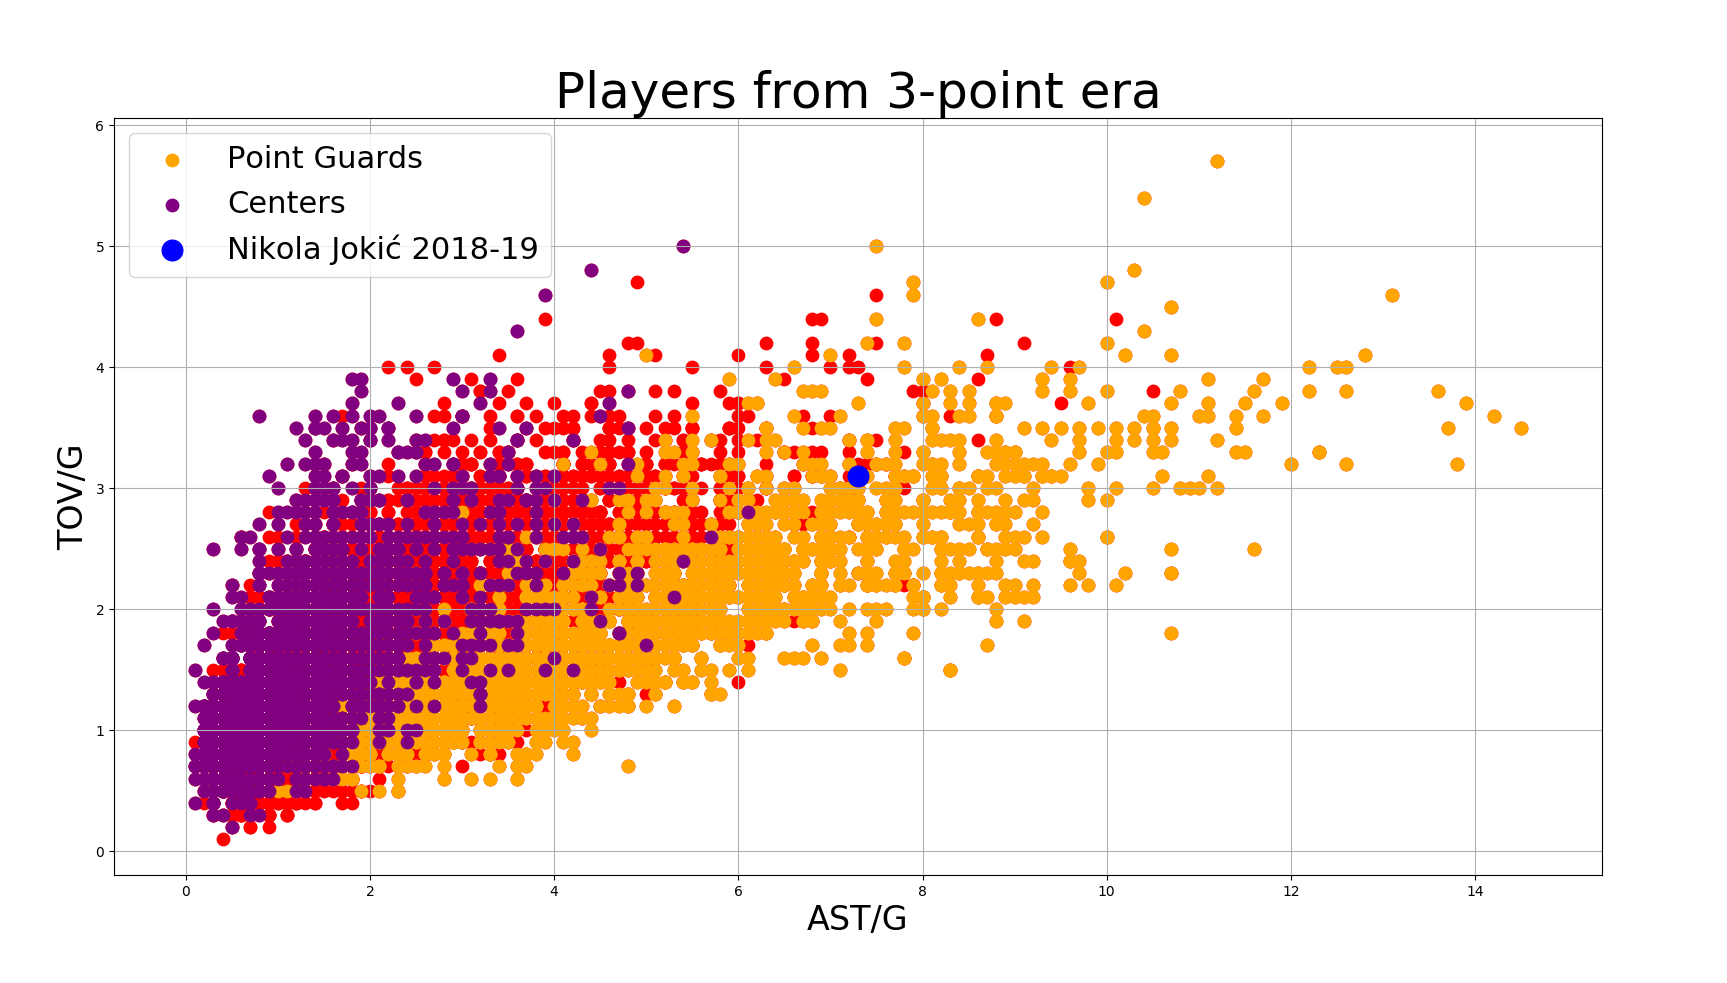
\includegraphics[scale=0.30]{ast_tov_g_3point_era.png}
\end{center}
\caption{AST\% to TOV\% for players from 3-point era (min 15 MP/G and 35 G)}
\label{plt:ast_tov_g_3p}
\end{figure}

On the second figure, that represents AST\% and TOV\% of the players from 3-point era, he moved down and right, which is good. Not only that, but it appears that there are fewer player between him and bottom-right corner than on the previous plot. That implies that his stats are a little bit better than what the per game numbers show.

\begin{figure}[h!]
\begin{center}
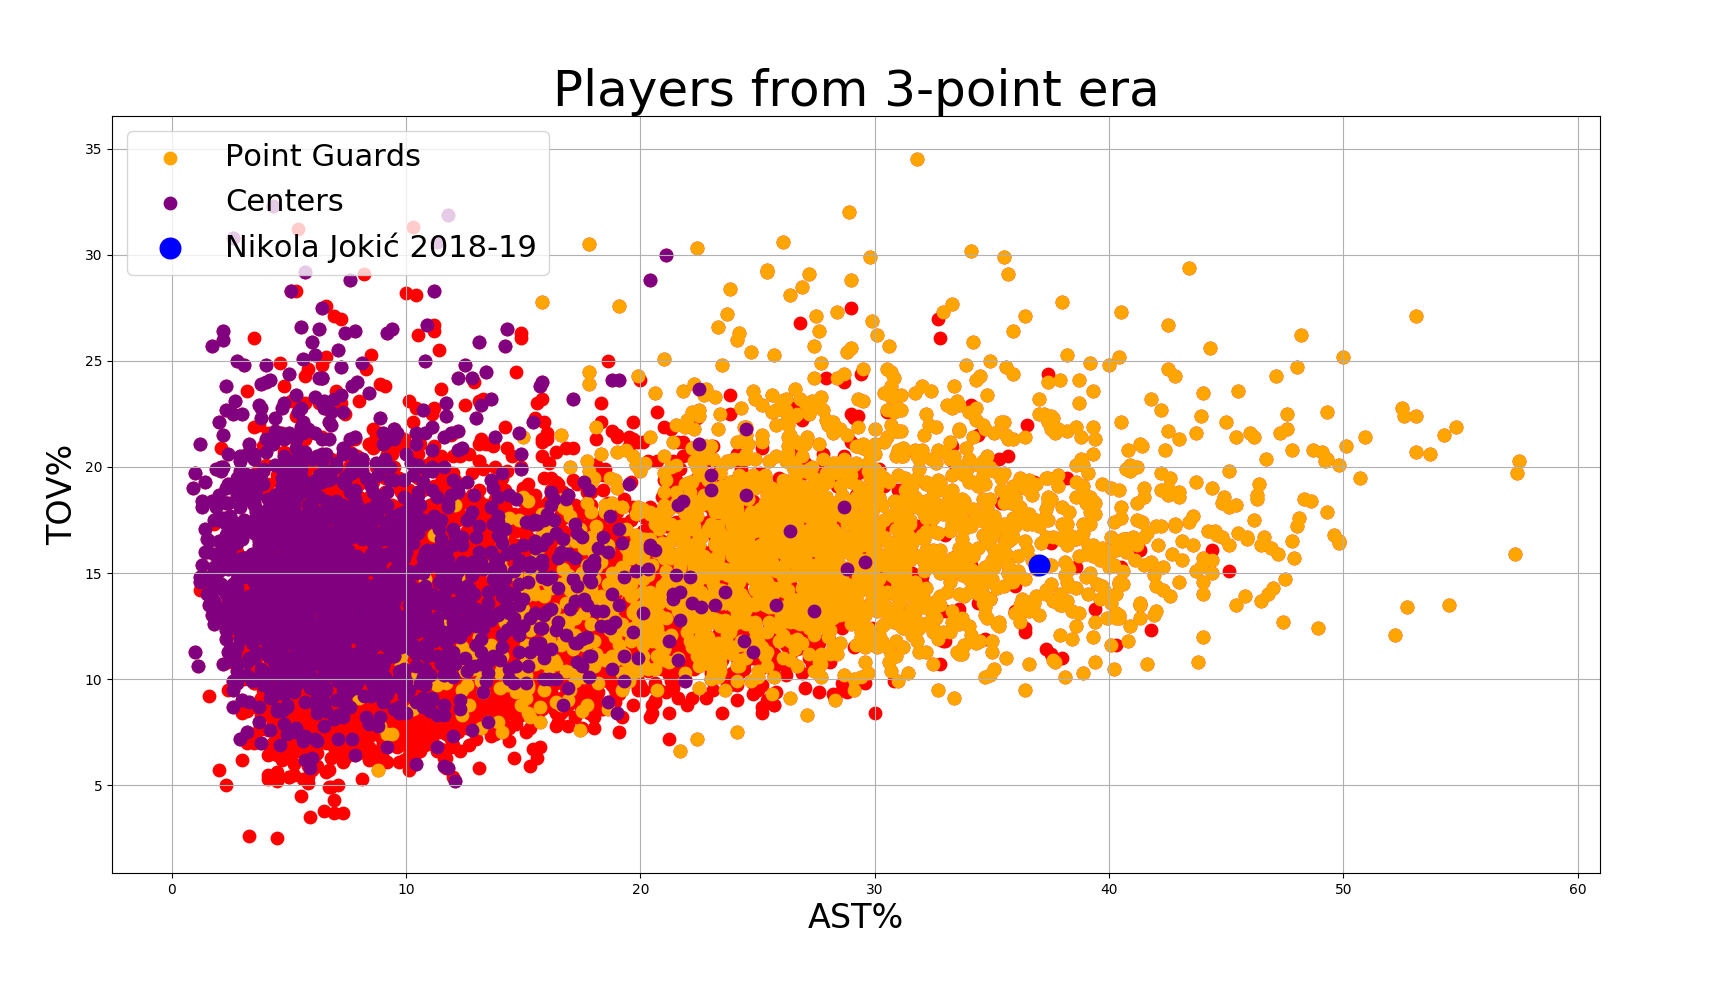
\includegraphics[scale=0.30]{ast_tov_pct_3point_era.png}
\end{center}
\caption{AST\% to TOV\% for players from 3-point era (min 15 MP/G and 35 G)}
\label{plt:ast_tov_pct_3p}
\end{figure}

To conclude this subsection, Nikola Joki\' c is absolutely best passing center ever. His passing numbers also look good when compared to the numbers of the elite passers, but are still inferior to them. Basically, he is passing like a starting caliber point guard. I am, personally, very excited for the future of Denver Nuggets.

\pagebreak

\section{Moreyball}
\label{sec:moreyball}

Moreyball, named after Houston Rockets General manager Daryl Morey, is an offensive strategy in basketball that is based on taking just the most efficient shots, the shots that are worth the most points per possession. Those shots are 3-point shots, shots close to the basket and free throws. Let's see why those shots are more efficient than others.

Average Offensive rating in 2018-19 season in the NBA was 110.4. That means that an average offense scores 110.4 points per 100 possessions. In that same season, percentages of shots from the areas calculated by distance from the basket, according to the stats.nba.com, were:

\begin{itemize}
	\item Percentage of shots close to the basket (less than 8 ft.) is 0.579. That translates to 115.8 points per 100 possessions.
	\item Percentage of shots from 8 to 16 ft. is 0.412. That translates to 82.4 points per 100 possessions.
	\item Percentage of shots from 16 to 24 ft. is 0.401. That translates to 80.2 points per 100 possessions.
	\item Percentage of shots at the 3-point line (24+ ft.) is 0.357, with back court shots excluded. That translates to 107.1 points per 100 possessions.
	\item Percentage of \textbf{wide open} 3-point shots (where the nearest defender is at 6+ ft.) is 0.380. That translates to 114.0 points per 100 possessions.
	\item Percentage of a free throw shot is 0.776. That translates to 76.6 points per 100 possessions (one shot), 153.2 per 100 (two shots) or 229.8 per 100 (three shots).
\end{itemize}

From here, it is easy to conclude which shots produce more points per possession than the average. Those shots are either close to the basket, or three-pointers. Not only that, but the most efficient field goal a team can take is the one from less than 8 feet, because those shots are hard to miss. Also, two free throws per possession are extremly efficient. Notice how staggering difference is beetween average 3-point shot and three free throws, the obvious reason why fouling someone on three-point shot is extremely bad.

Because of that, most teams nowdays are trying to implement Moreyball. If we compare shootcharts by teams from 2018-19 season, and shotchart from the same team just 6 years prior (2012-13 season), we will se noticable difference (figure \ref{plt:shotcharts}). Teams used to shoot more mid-range shots.

\begin{figure}[h!]
\begin{center}
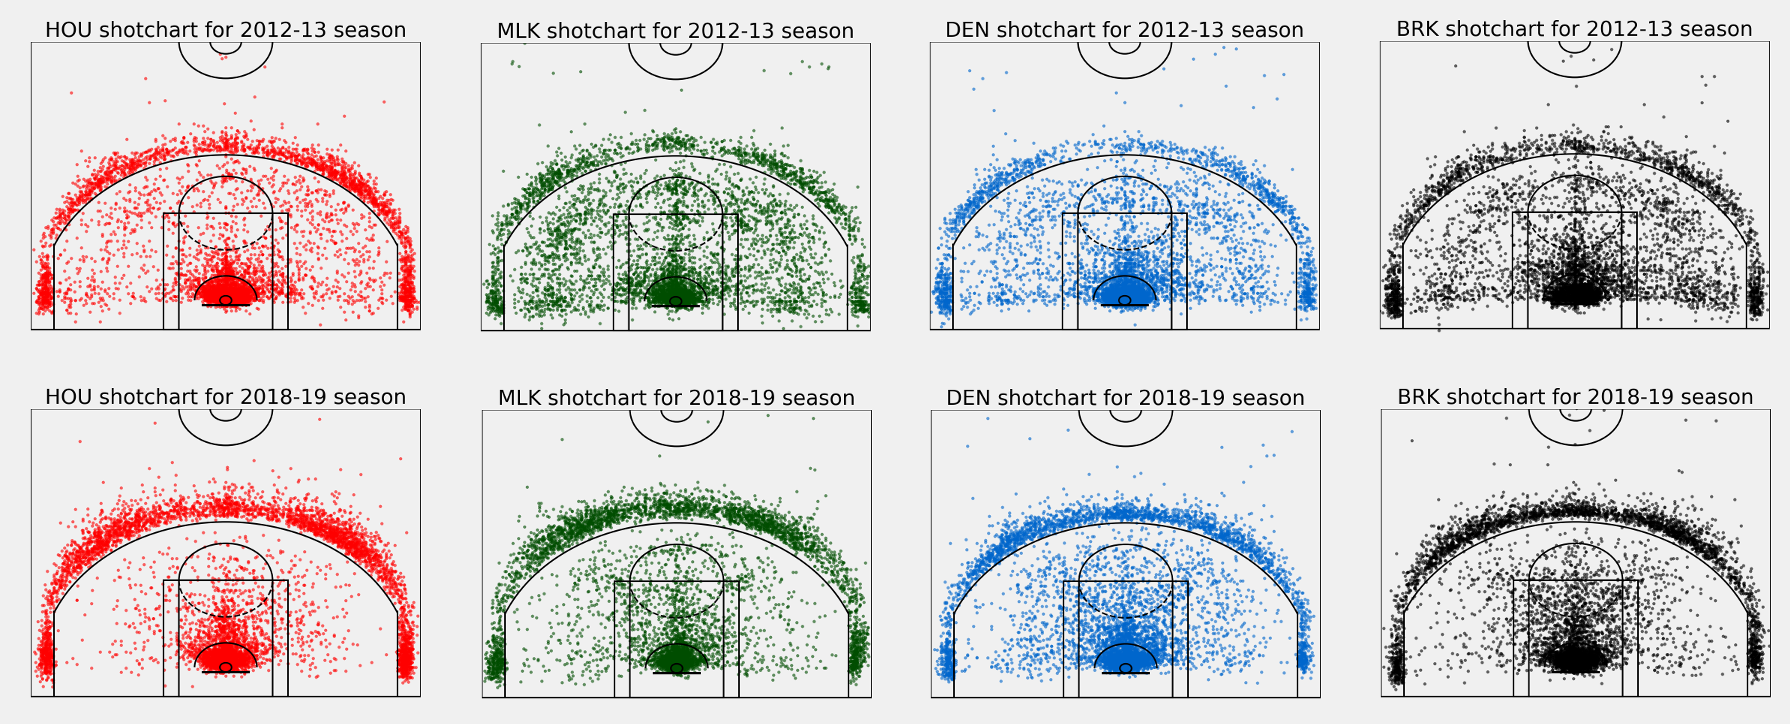
\includegraphics[scale=0.27]{shotcharts.png}
\end{center}
\caption{Shotcharts from 2012-13 and 2018-19 seasons}
\label{plt:shotcharts}
\end{figure}

Team that popularized Moreyball, Houston Rockets, were last in number of mid-range attempts in 2018-19 season. They finished as a 2nd best offense in the league, just 0.4 points per 100 possessions behind 1st ranked Golden State Warriors. They were one of the best offensive teams for a while, finishing top 2 in ORtg in 2016-17 (2nd), 2017-18 (1st) and 2018-19 (2nd) seasons. Not only that, but from the 2012-13 season, they missed top 7 in ORtg only once, in 2014-15 (ranked 12th).

So, Moreyball should work, right? I mean, if a team is shooting just shots that are more efficient than the average, or in other words drastically decrease number of mid-range shots, it will have above average offense. Let's compare ORtg to a percentage of shots that were mid-range, teams took in a 2018-19 season.

\begin{figure}[h!]
\begin{center}
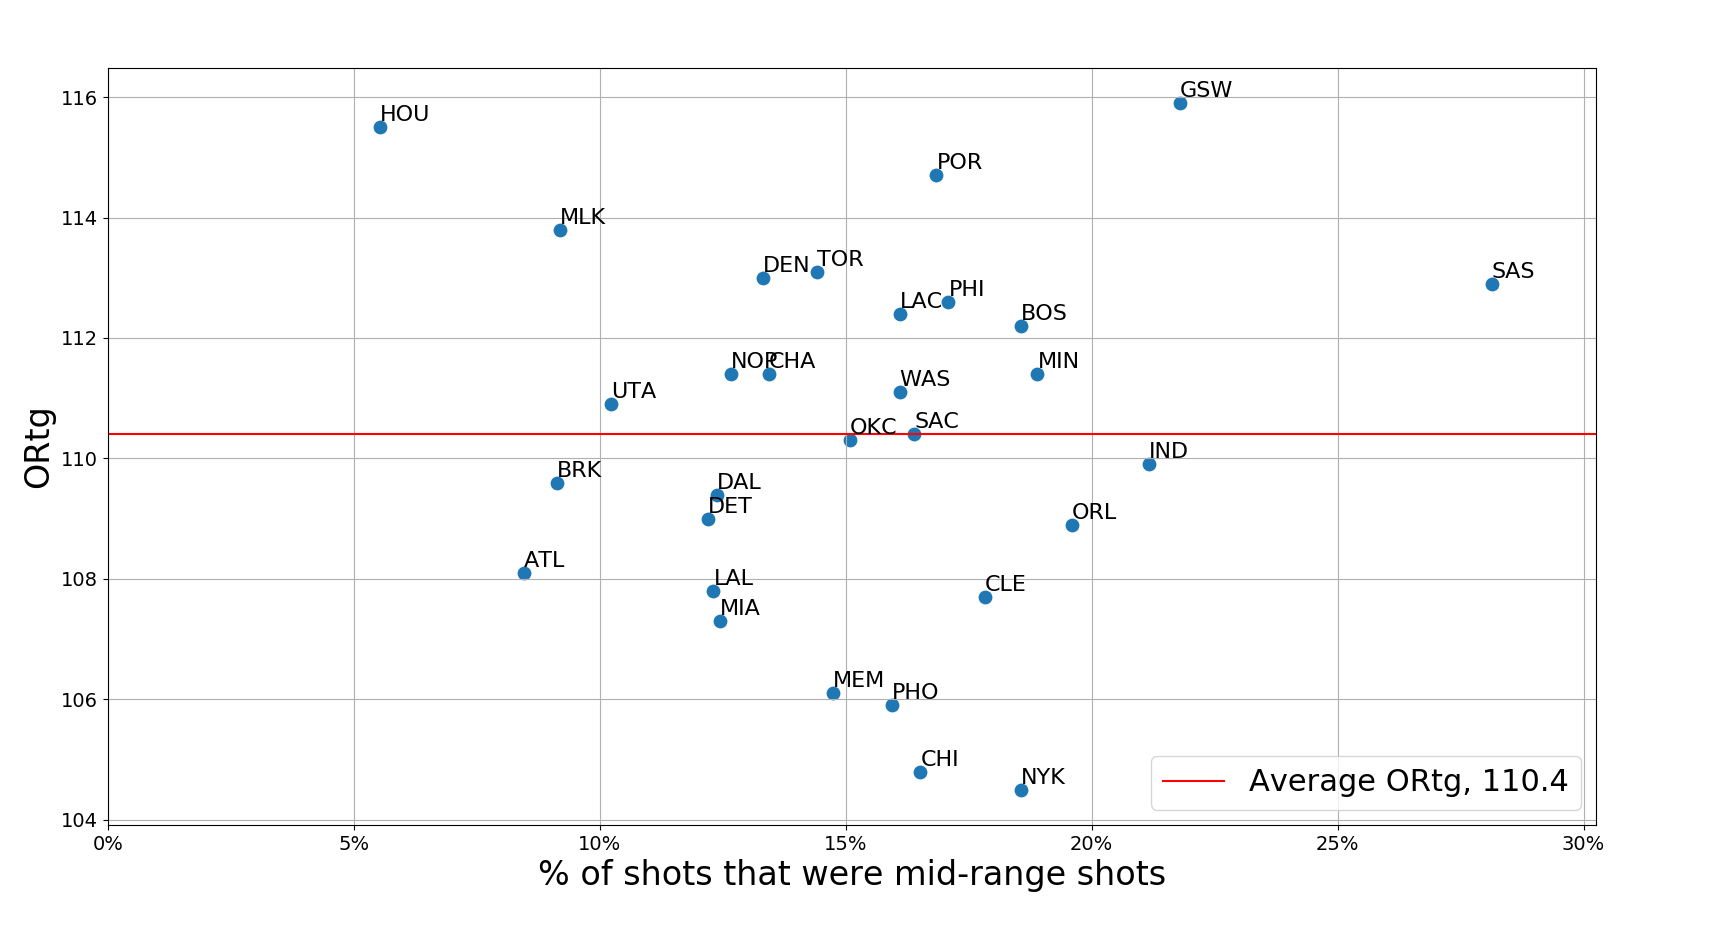
\includegraphics[scale=0.29]{ortg_pct_mid_range.png}
\end{center}
\caption{ORtg to \% of shots that were mid-range by team (2018-19 season)}
\label{plt:ortg_oct_mid_range}
\end{figure}

The results are interesting. Team with the best ORtg, Golden State Warriors, was second in percentage of mid-range shots, while the second-placed Houston was dead last in that category. San Antonio Spurs, team that was first in percentage of mid-range shots, had 7th best offense. Teams such as Atlanta (23rd), Brooklyn (19th) and Milwaukee (4th), beside Houston, had taken less than 10\% of their shots from mid-range, with significant difference in ORtg. So, implementing Morreyball might not produce above average offense, and not only that, but an offense with lot of, usually inefficient, mid-range shots can work well (if a team has efficient mid-range scorer). If that's the case, why would teams even try to play Moreyball?

Because Morreyball leads to a more efficient offence in general! Take a look at table \ref{tab:seasons_comp}. Every season shown has increase of three-point attempt rate from the season before, and with it, better ORtg and better efficiency.

\begin{table}[h!]
\begin{center}
\begin{tabular}{|l|c|c|c|c|c|} \hline
\textbf{Stat \textbackslash Season} & \textbf{2000-01} & \textbf{2005-06} & \textbf{2010-11} & \textbf{2015-16} & \textbf{2018-19} \\ \hline
\textbf{TS\%} & 51.8\% & 53.6\% & 54.1\% & 54.1\% & 56.0\% \\ \hline
\textbf{ORtg} & 103.0 & 106.2 & 107.3 & 106.4 & 110.4 \\ \hline
\textbf{Mid-range attempt freq} & 23\% & 23.6\% & 21.4\% & 16.2\% & 9.2\% \\ \hline
\textbf{3P attempt freq} & 17\% & 20.2\% & 22.2\% & 28.5\% & 35.9\% \\ \hline
\end{tabular}
\caption{Comparing stats through seasons}
\label{tab:seasons_comp}
\end{center}
\end{table}

Correlations on data from season 2000-01 to season 2018-19 (from basketball-reference.com) are showing same results:

\begin{itemize}
	\item Correlation between TS\% and ORtg: 0.967
	\item Correlation between TS\% and \% of 3PA: 0.851
	\item Correlation between TS\% and \% of mid-rangea ttempts: -0.733
	\item Correlation between \% of 3PA and ORtg: 0.766
	\item Correlation between \% of mid-range attempts and ORtg: -0.634
\end{itemize}

Results are, based on everyting we have seen so far, expected. There is a very strong correlaton between efficiency and ORtg. True shooting percentage depends more on frequency of 3-point shots than on frequency of mid-range shots. More three-pointers, better efficiency, but also fewer mid-range shots, better efficiency, just not to the same degree. These are just some extra reasons why Moreyball does produce more points per possession!

To conclude, Moreyball produces more points per possession in general, but offenses that are more Moreyball than the others, might not be above average on a season level. Rise in Moreyball contributed to the rise in ORtg in recent years. Also, let's note that strategies with lot of mid-range shooting can produce good/above average offense. % maybe why?


\section{Clustering}
\label{sec:clustering}

In this secion I will try to, via clustering, find interesting things in NBA data. Clustering is process of finding different groups in data, where element in one group is more similar to another element in the same group than to any element from any other group \cite{clustering}. Those groups are called \textbf{clusters}. Two algorithms will be used.

First one is \textbf{K-Means clustering.} This algorithm will find \textbf{K} groups. Every group will be represented by one point, called \textit{centroid}. Point that is not a centroid will belong to the cluster that is represented by the closest centroid to it. Algotihm will first choose K centroids at random, and then preform iterative calculations to optimize positions of said centroids. User can choose number of iterations. Because centroids are initialized at random, algorithm should be performed muliple times. Thenm out of all results, the best one is chosen. \cite{clustering}

Second is \textbf{Hierarchichal clustering.} There are two types, Divisive and Agglomerative clustering. Former method begins with one cluster that contains every data point. Then, iteration by iteration, it will split that cluster in smaller ones, by similarity, until every point is cluster for itself. Latter is the opposite. It will start with as many clusters as data points, and then, iteratively, it will group two that are the most similar into one group, until only one cluster, that contains every data point, remains. \cite{clustering}

Similarity between clusters is calculated by \textbf{linkage}. In \textit{single} linkage, the smaller the distance between closest points of two clusters is, the more similar they are. \textit{Complete} linkage is the opposite, it takes into account distance between the farthest points of two clusters. The closer they are the the similarity between clusters in greater. \textit{Average} linkage takes into account average distance from any point that belongs to one cluster to any point that belongs to the other cluster. The smaller the distance, the more similar they are. The last one is \textit{Ward's} linkage. Similar to previous one, but instead of average, it calculates sum of squared distances. \cite{clustering}\cite{hierarchical}

One of the metrics that can tell if the clustering is good or not is \textbf{silhouette score}, calculated as $ (b - a)  / max(a, b) $, where \textit{a} is average distance to other data point in the same cluster, \textit{b} is average distance to other data point in the nearest cluster. Valus of this score can go from -1 to 1. The higher value the better. \cite{clustering}

\subsection{Determining player's roles by games played}
\label{subsec:players_roles}

Player in the NBA usually can be placed in one of the three categories, starter, bench player and non-rotational player. First group, starters, are expected to start every game they play. Starters play the most minutes per game. They might not play every game due to various injuries and rest days. Also, they might not start evey game. For example, starter might get injured, and when he is healed coach might not put him in the starting lineup. That is usually practice if the starter is on a minute restriction, meaning he will play in the game, but will play in the fewer minutes than he usually plays in when he starts. Second group are bench players. They are not usually starters, but are important for the success of the team. They play in a lot of minutes, but not as much as starters. Bench players might get to start some games because starter is injured, or maybe because of matchups, but that is not really likely. Third are non-rotational players. They aren't usually playing in the game, or if they are, they are playing small amount of minutes or garbage time. Note that these players also might even start some games, if team has serious problem with injuries. Also, it's possible that a player make progress or regress during a season, which will result in promotion or demotion.

The starting point is clustering based on games played (\textbf{G}) and games started (\textbf{GS}). It is expected that players with small amount of games are the non-rotational ones, the ones that started lot of games are startes and the others are bench players. Data is shown of figure \ref{plt:g_gs} and represents players from 2018-19 season. I beleve that the biggest difference between results of clustering algorithms will be in the area in the middle of the diagonal, where players did start every (or almost every) game they played in, but maybe didn't play enough games to be considered starters.

\begin{figure}[h!]
\begin{center}
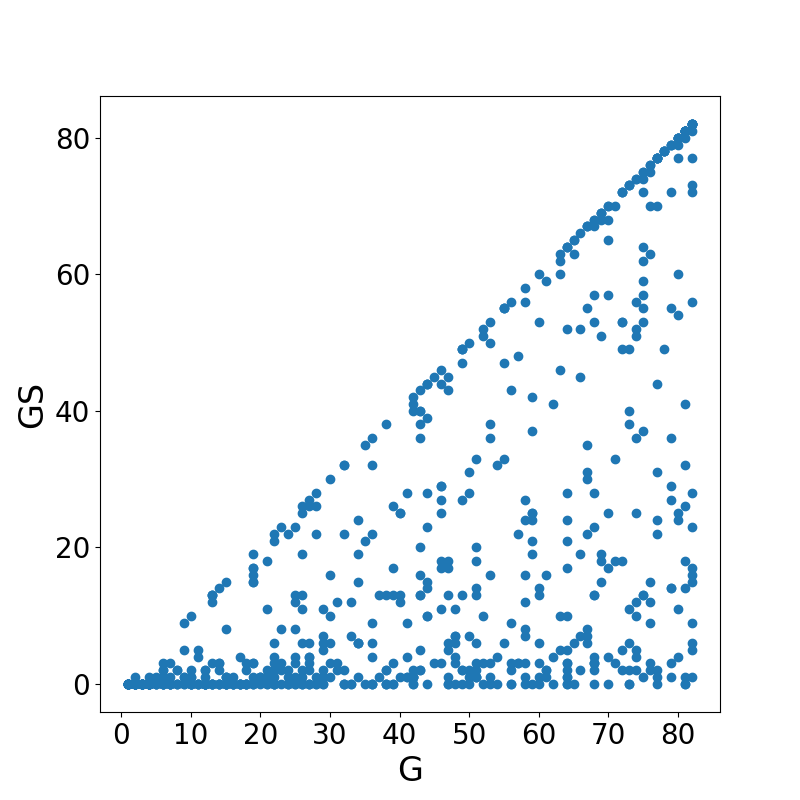
\includegraphics[scale=0.3]{g_to_gs.png}
\end{center}
\caption{Games played to Games started (2018-19 season)}
\label{plt:g_gs}
\end{figure}

The first clustering algorithm is KMeans. Value of K is 3 because players are supposed to be grouped in three groups. After that, I tried hierarchichal clustering methods with simple, complete, average and Ward's linkage. Results can be found in table \ref{tab:clust_score_k3}.

\begin{table}[!h]
\begin{center}
\begin{tabular}{|l|c|} \hline
\textbf{Clustering method} & \textbf{Silhouette score}  \\ \hline
KMeans & 0.550  \\ \hline
Hierarchichal, simple linkage & -0.007  \\ \hline
Hierarchichal, complete linkage & 0.524  \\ \hline
Hierarchichal, average linkage &  0.519  \\ \hline
Hierarchichal, Ward's linkage & 0.495  \\ \hline
\end{tabular}
\caption{Silhoutte score for G and GS}
\label{tab:clust_score_k3}
\end{center}
\end{table}

Judging by the silhouette score, clusters arn'ts be well defined, which could also be assumed from the previous plot. Method with the best score is KMeans.
Let's take a look at the results (figure \ref{plt:clust_g_gs_k3}).

\begin{figure}
\centering
\begin{minipage}{.22\textwidth}
  \centering
  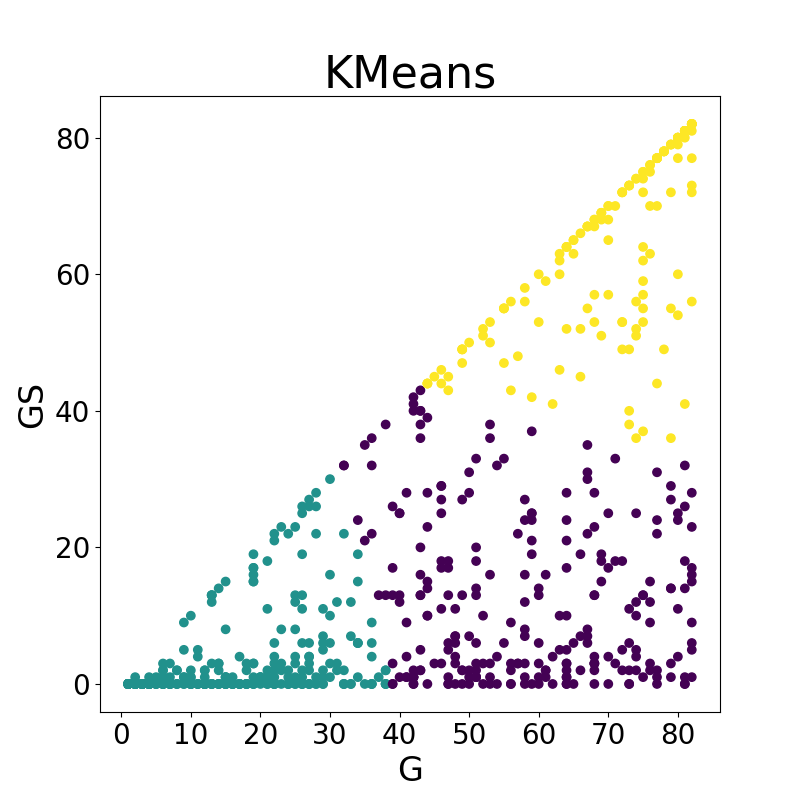
\includegraphics[scale=0.14]{kmeans_g_gs.png}
  \label{fig:kmeans_g_gs}
\end{minipage}
\begin{minipage}{.22\textwidth}
  \centering
  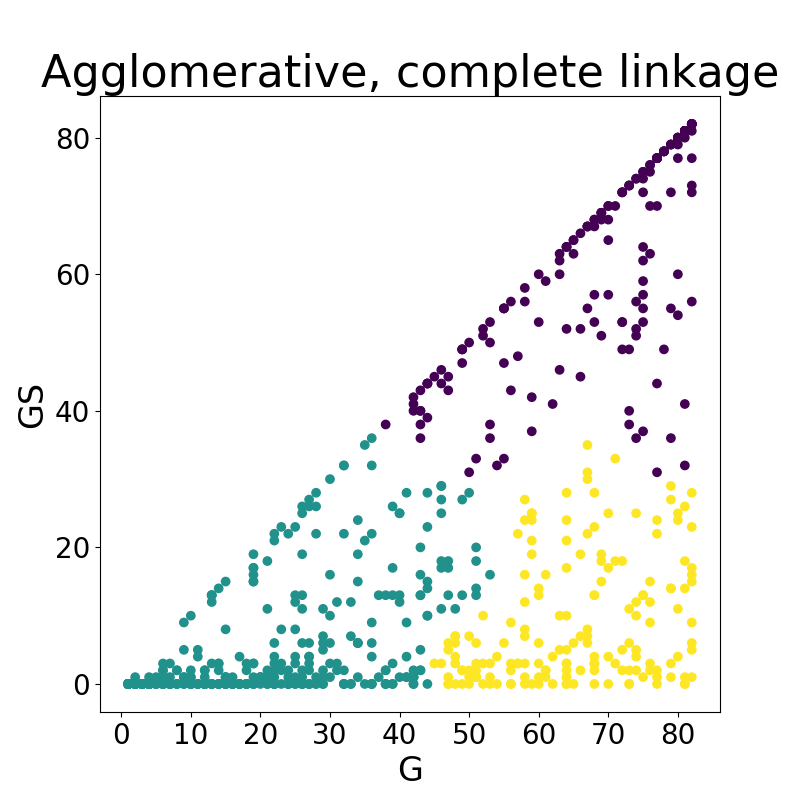
\includegraphics[scale=0.14]{complete_link_g_gs.png}
  \label{fig:complete_g_gs}
\end{minipage}
\begin{minipage}{.22\textwidth}
  \centering
  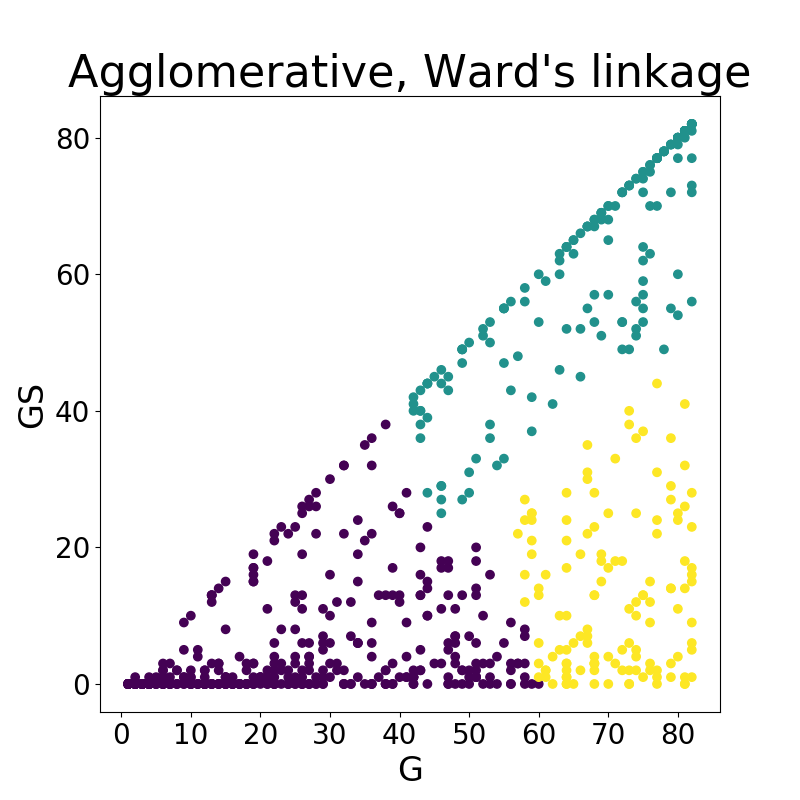
\includegraphics[scale=0.14]{ward_link_g_gs.png}
  \label{fig:ward_g_gs}
\end{minipage}
\begin{minipage}{.22\textwidth}
  \centering
  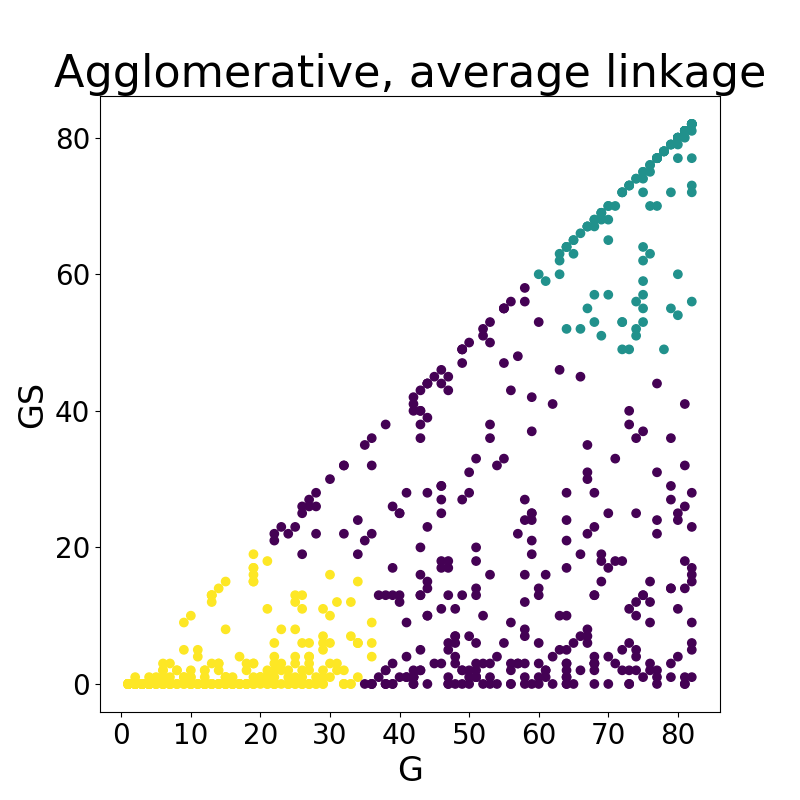
\includegraphics[scale=0.14]{average_link_g_gs.png}
  \label{fig:average_g_gs}
\end{minipage}
\caption{Clusters on G and GS data}
\label{plt:clust_g_gs_k3}
\end{figure}

The results are somewhat expected. In the upper right corner is the cluster that contains starters. In the lower left are players that are outside of rotation while bench players are in between. KMeans and agglomerative with average linkage are somewhat similar, where players in the middle of the diagonal are considered bench players. In the other two, those players are staters.

Maybe the clustering will have better results if we add one more variable, minutes played (\textbf{MP}). It is expected that starters play the most minutes per game, while players that are outside of rotation play the least, if any. Bech players should play, but not as much as starters. Also, note that values of MP per game, for 2018-19 season, are between 0 and 36.9, the amount of minutes the league leaders, Bradley Beal and Paul George, played per game. Values of G and GS are from 0 to 82. Because of that, it is possible that normalazing data (scaling to [0, 1] interval) before clustering might improve results. As we have already seen, because of the data, clusters cannot really be well defined, so the part with silhouette score is skipped. Results for non-scaled data are shown in the figure \ref{plt:clust_g_gs_mp_k3} while results for scaled data are in figure \ref{plt:clust_g_gs_mp_k3_scaled}. Note that clusters are still shown in G to GS plot, even with MP variable included in clusering. The reason behind this is comparing results with the previous one.

\begin{figure}
\centering
\begin{minipage}{.22\textwidth}
  \centering
  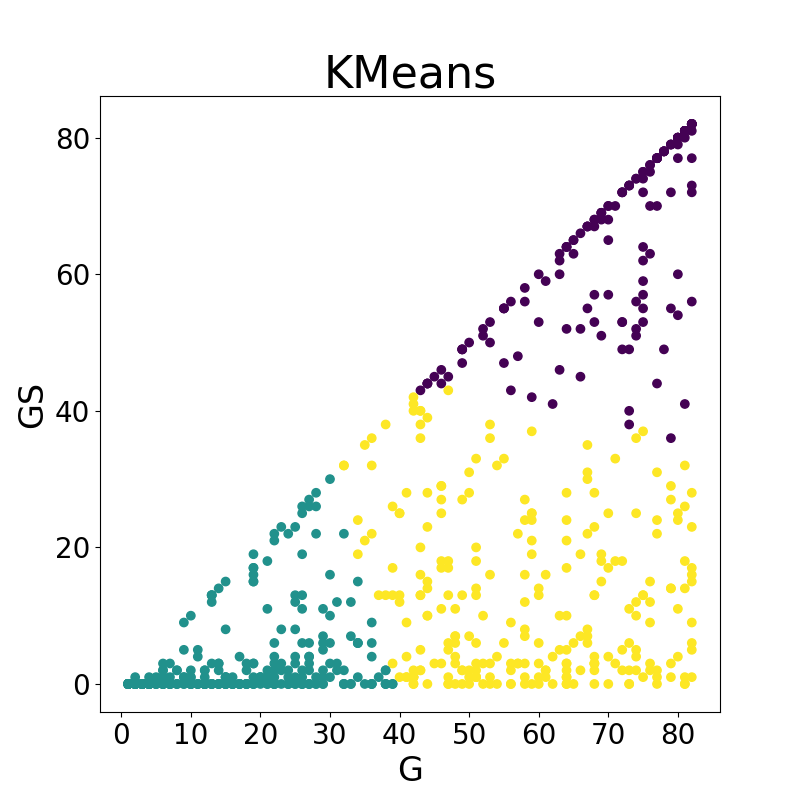
\includegraphics[scale=0.14]{kmeans_g_gs_mp.png}
  \label{fig:kmeans_g_gs_mp}
\end{minipage}
\begin{minipage}{.22\textwidth}
  \centering
  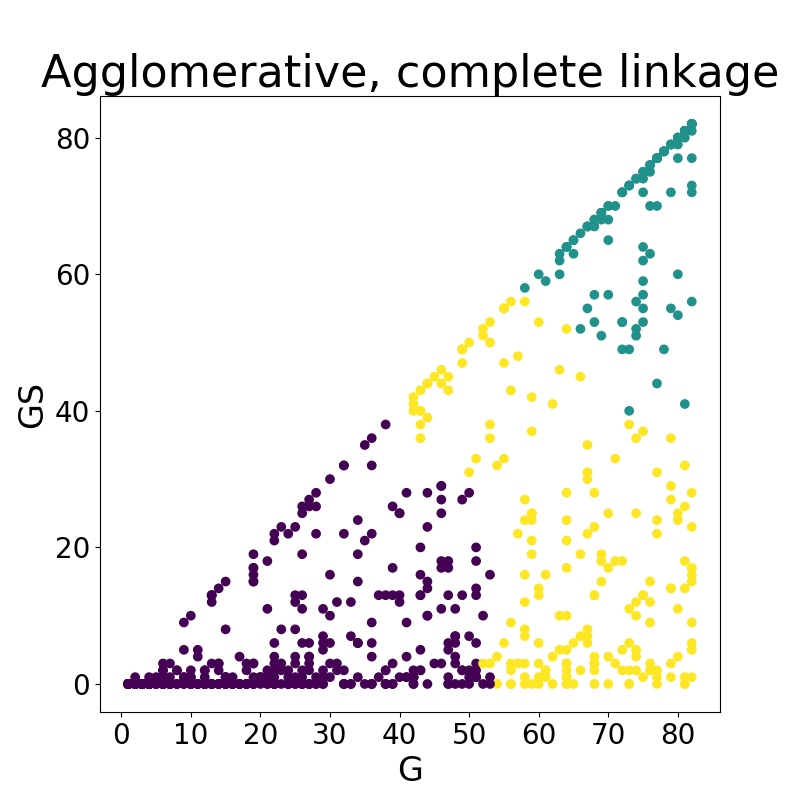
\includegraphics[scale=0.14]{complete_link_g_gs_mp.png}
  \label{fig:complete_g_gs_mp}
\end{minipage}
\begin{minipage}{.22\textwidth}
  \centering
  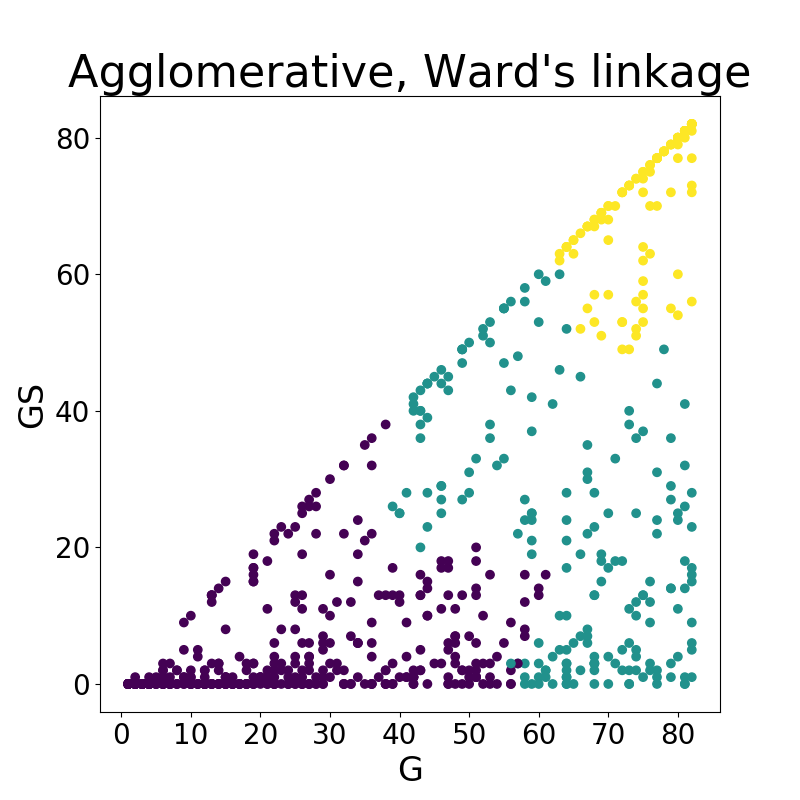
\includegraphics[scale=0.14]{ward_link_g_gs_mp.png}
  \label{fig:ward_g_gs_mp}
\end{minipage}
\begin{minipage}{.22\textwidth}
  \centering
  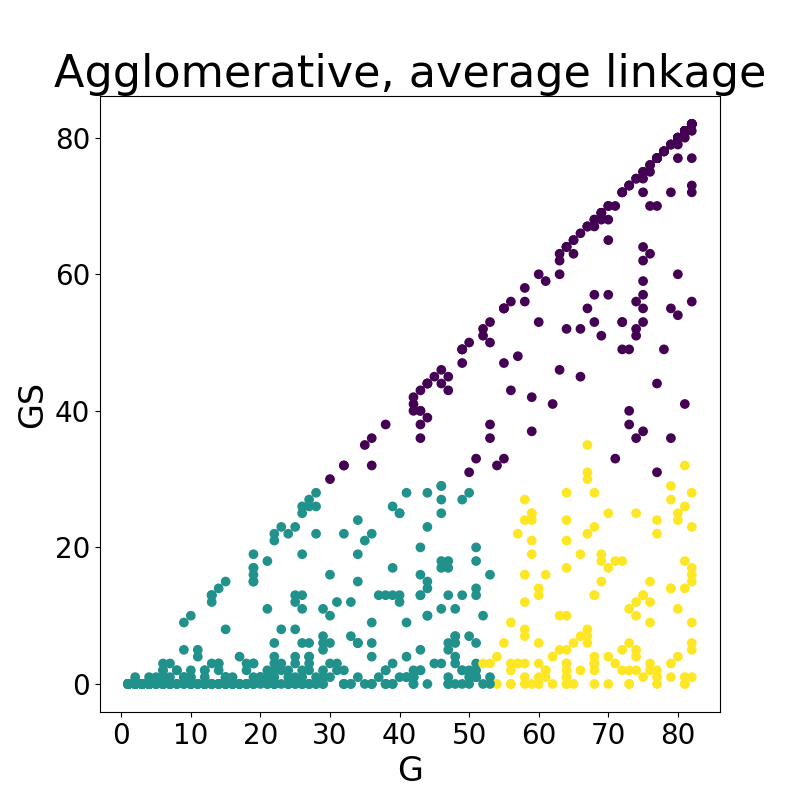
\includegraphics[scale=0.14]{average_link_g_gs_mp.png}
  \label{fig:average_g_gs_mp}
\end{minipage}
\caption{Clusters on G, GS and MP data}
\label{plt:clust_g_gs_mp_k3}
\end{figure}

KMeans algorithm have almost the same results as before, while others are different. The main difference is, unsurprisingly, middle of the diagonal. As opposed to before, agglomerative with complete and Ward's linkage are grouping it with bench players. Agglomerative with average linkage changed the most. with middle of the diagonal in starters group. Maybe scaled data will have better results.

\begin{figure}
\centering
\begin{minipage}{.22\textwidth}
  \centering
  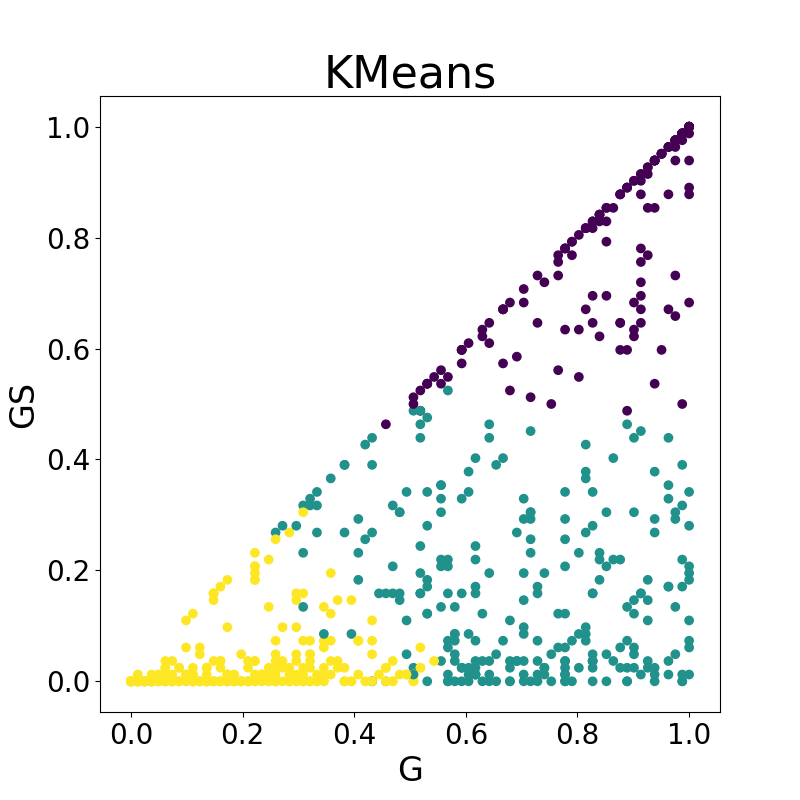
\includegraphics[scale=0.14]{kmeans_g_gs_mp_scaled.png}
  \label{fig:kmeans_g_gs_mp_scaled}
\end{minipage}
\begin{minipage}{.22\textwidth}
  \centering
  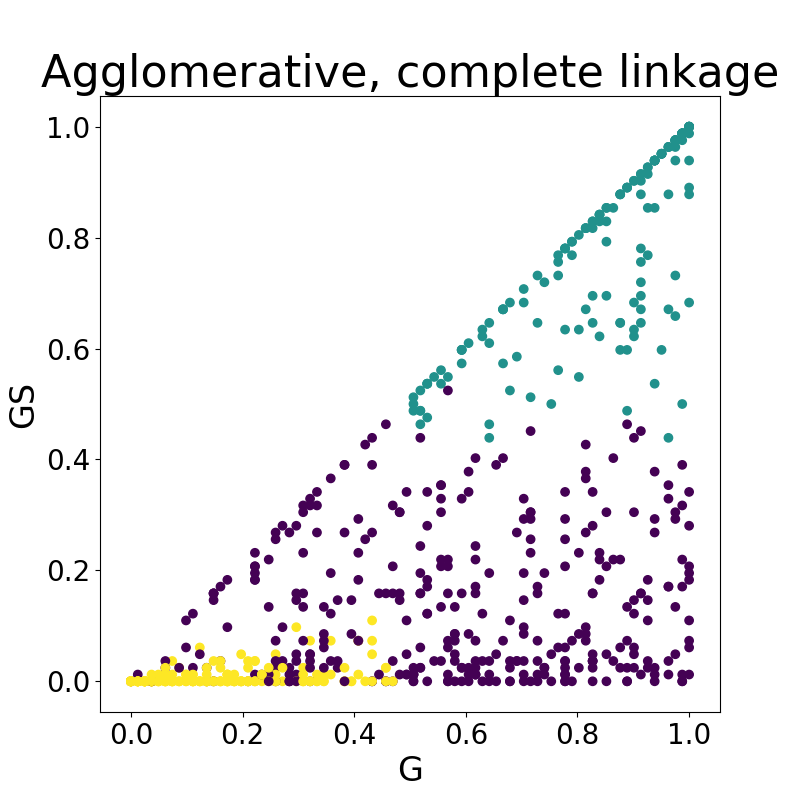
\includegraphics[scale=0.14]{complete_link_g_gs_mp_scaled.png}
  \label{fig:complete_g_gs_mp_scaled}
\end{minipage}
\begin{minipage}{.22\textwidth}
  \centering
  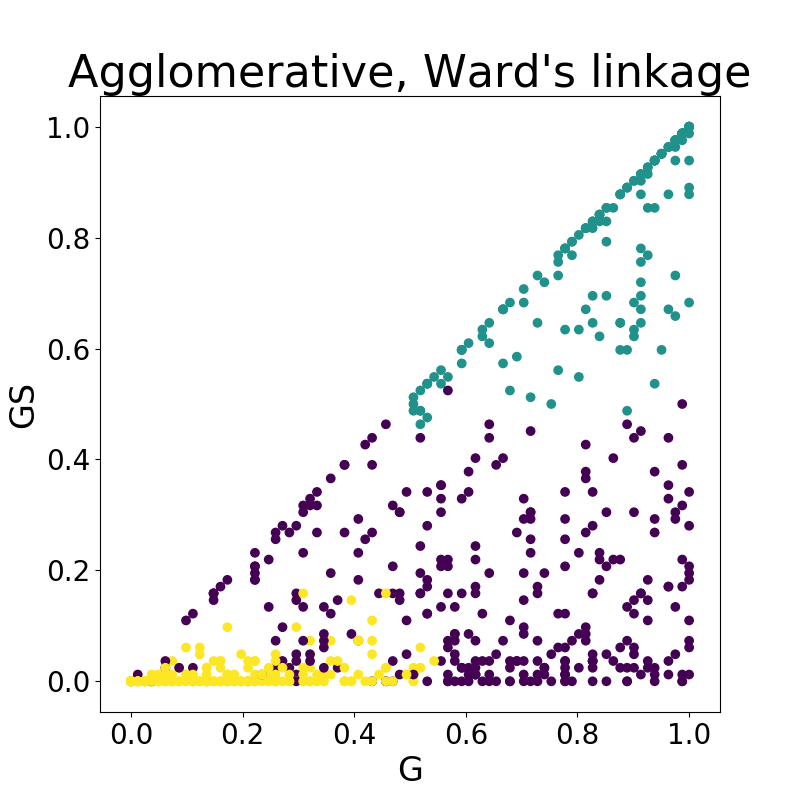
\includegraphics[scale=0.14]{ward_link_g_gs_mp_scaled.png}
  \label{fig:ward_g_gs_mp_scaled}
\end{minipage}
\begin{minipage}{.22\textwidth}
  \centering
  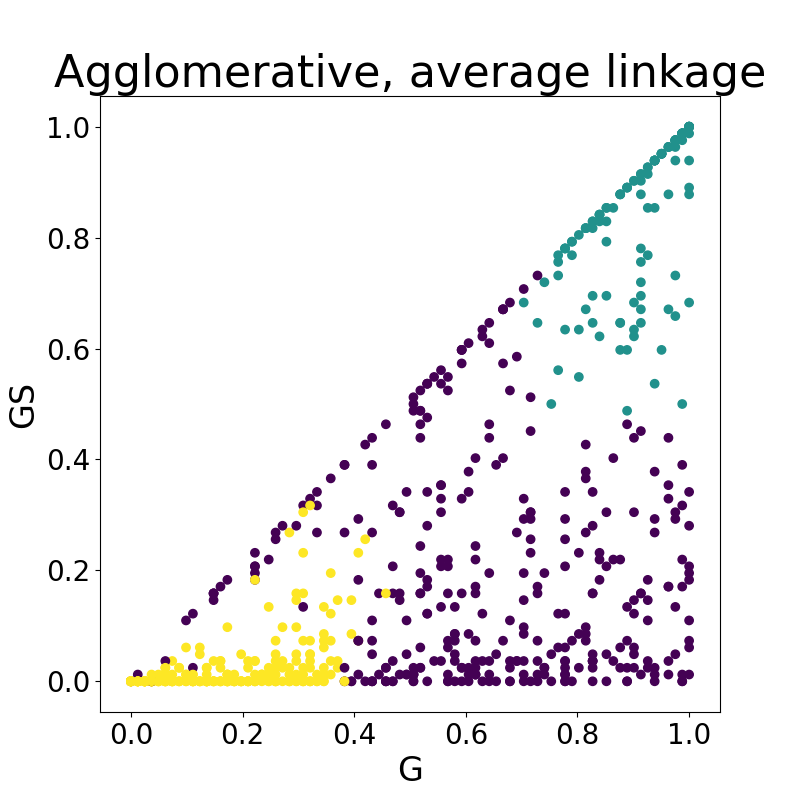
\includegraphics[scale=0.14]{average_link_g_gs_mp_scaled.png}
  \label{fig:average_g_gs_mp_scaled}
\end{minipage}
\caption{Clusters G, GS and MP scaled data}
\label{plt:clust_g_gs_mp_k3_scaled}
\end{figure}

Scaling data definitely gave us different results, although results from KMeans are still similar to the previous ones. The biggest difference can be observed in cluster with non-rotational players. Players in that cluster played around half of the games, but did not start in almost any of them. Because of that, cluster with bench players increased in size. Cluster with starters remained somewhat same.

Clusters with starters were upper right, clusters with non-rotational players were lower left, and clusters with bench players were lower right, as expected. There were different results in clustering of the middle of the diagonal, that usually belonged in starters or bench players. There is a case to be made for both, but I am personally more leaning towards starters option. That part of the diagonal contains players that played somewhere between 40 and 55 games, and started in a lot of them (or almost all of them). Notable players from that group are LeBron James, Brandon Ingram, Wayne Ellington, Wendell Carter, Lonzo Ball, Tristan Thompson, Will Barton, Rajon  etc. I would personally count them into starters, who missed significant part of the season due injuries. I liked results of agglomerative clustering with Ward's linkage on games and games started data, although I would argue that more players from non-rotational players cluster should belong to the bench cluster, specifically the ones that played more than 40 games.

\pagebreak

\addcontentsline{toc}{section}{References}
\appendix
\bibliography{ref}
\bibliographystyle{unsrt}
\appendix

\end{document}
